\documentclass[a4paper, 10pt]{article}
\usepackage[left=2.5cm,bottom=2.5cm,right=2.5cm,top=2.5cm]{geometry}
\usepackage{amsmath,amssymb,mathtools, gensymb} 
\usepackage{booktabs} 
\usepackage{color}
\usepackage{longtable, lscape}
\usepackage{threeparttable}
\usepackage{caption}
\usepackage{verbatim, makecell}
\usepackage{subcaption}
\usepackage{float}
\renewcommand{\topfraction}{1}
\renewcommand{\bottomfraction}{1}
\floatstyle{plaintop}
\restylefloat{table}
\usepackage[section]{placeins}
\usepackage{url}
\usepackage[hidelinks]{hyperref}

\newcommand{\notes}[1]{\vspace{0.2cm} \caption*{ \scriptsize \textbf{Notes:} {#1}} }

% Add float barrier to subsections
\makeatletter
\AtBeginDocument{%
  \expandafter\renewcommand\expandafter\subsection\expandafter{%
    \expandafter\@fb@secFB\subsection
  }%
}
\makeatother

\renewcommand{\floatpagefraction}{1}


\title{Impact of diesel bans on traffic flows}

\begin{document}

\maketitle

%%%%%%%%%%%%%%%%%%%%%%%%%%%%%%%%%%%%%%%%%%%%%%%%%%%%%%%%%%%%%%%%%%%
\color[rgb]{0,0,0}
\section{Berlin traffic data}

Traffic monitor locations (MQ - Messquerschnitt) with separate detectors (DET - detektors) for each lane $\rightarrow$ focus on monitor locations, 2016 - 2021

\begin{itemize}
   \item tag - Datum
   \item stunde - Stunde des Tages für die die Messwerte ermittelt wurden (8 => 08:00 - 08:59).
   \item qualitaet - gibt den Anteil der für die Stunde vorliegenden einwandfreien Messintervalle wieder: 1.0 = 100\%
   \item Anzahl aller Kraftfahrzeuge in der Stunde.
   \item Anzahl aller Pkw in der Stunde.
   \item Anzahl aller Lkw in der Stunde.
	 \item Mittlere Geschwindigkeit [km/h] über alle Kraftfahrzeuge in der Stunde.
   \item Mittlere Geschwindigkeit [km/h] über alle Pkw in der Stunde.
   \item Mittlere Geschwindigkeit [km/h] über alle Lkw in der Stunde.
\end{itemize}

\begin{figure}[!htb]
\centering
\caption{Monitors and diesel bans in Berlin}
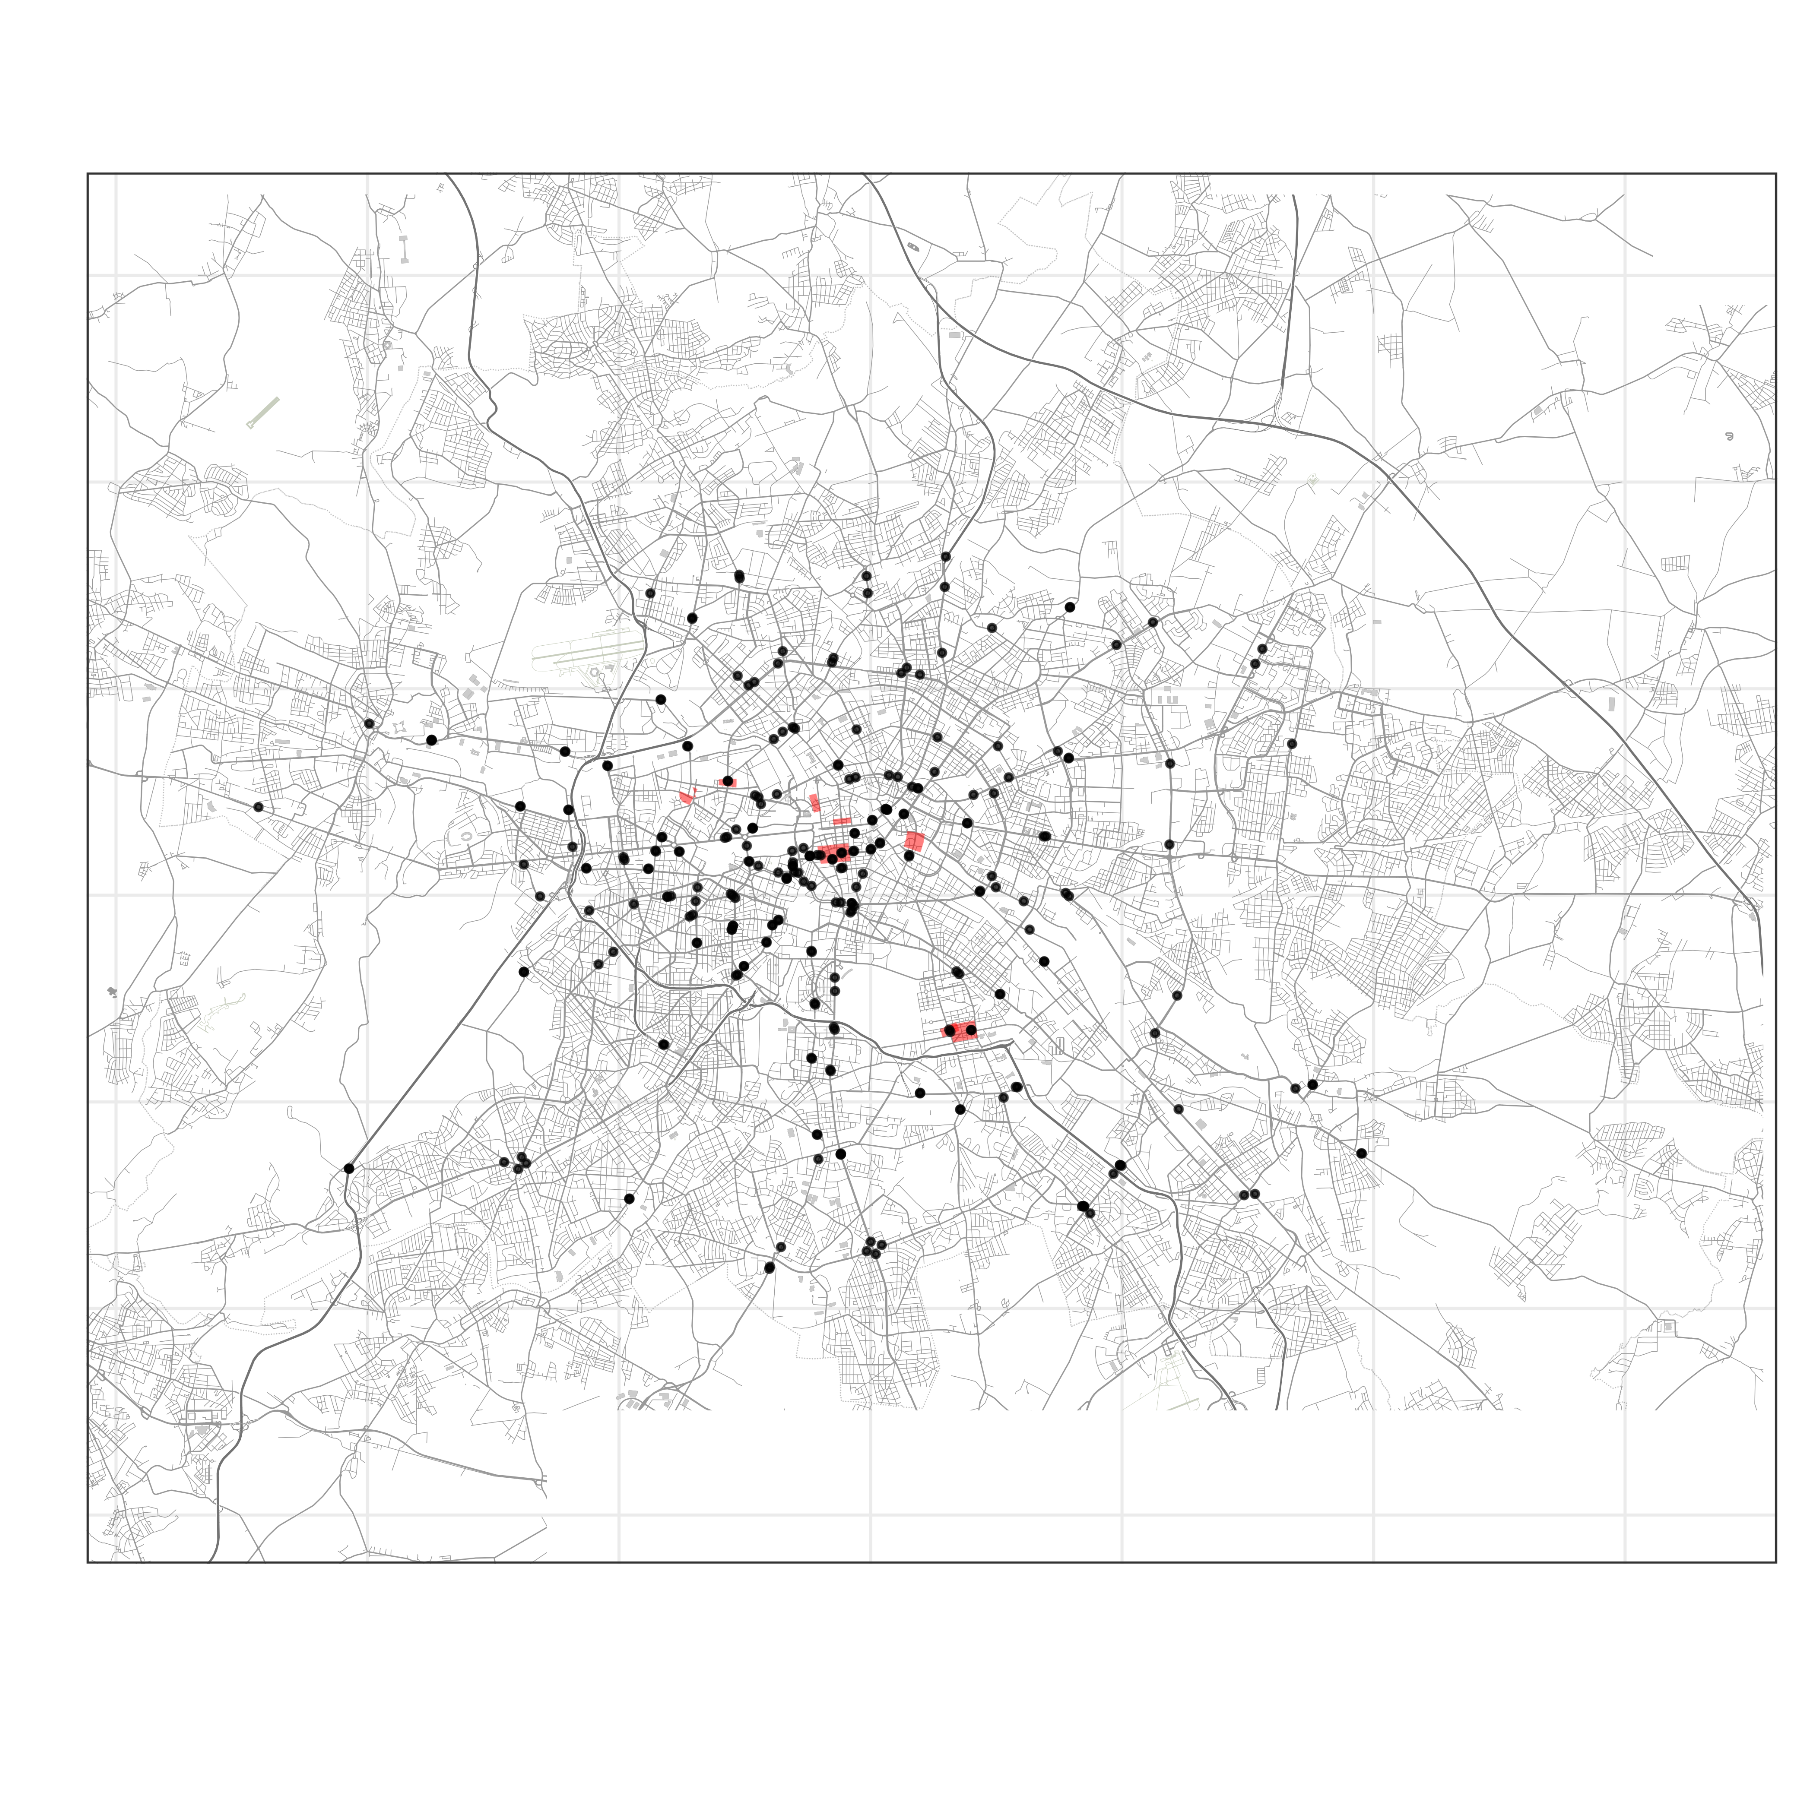
\includegraphics[width = \textwidth]{../04_figures/map_Berlin.png}
\end{figure}

%%%%%%%%%%%%%%%%%%%%%%%%%%%%%%%%%%%%%%%%%%%%%%%%%%%%%%%%%%%%%%%%%%%%
\clearpage\FloatBarrier
\subsection{Hourly data}
%
\begin{figure}[!htb]
\centering
\caption{Number of monitor locations (MQs) and sum of vehicles per month}
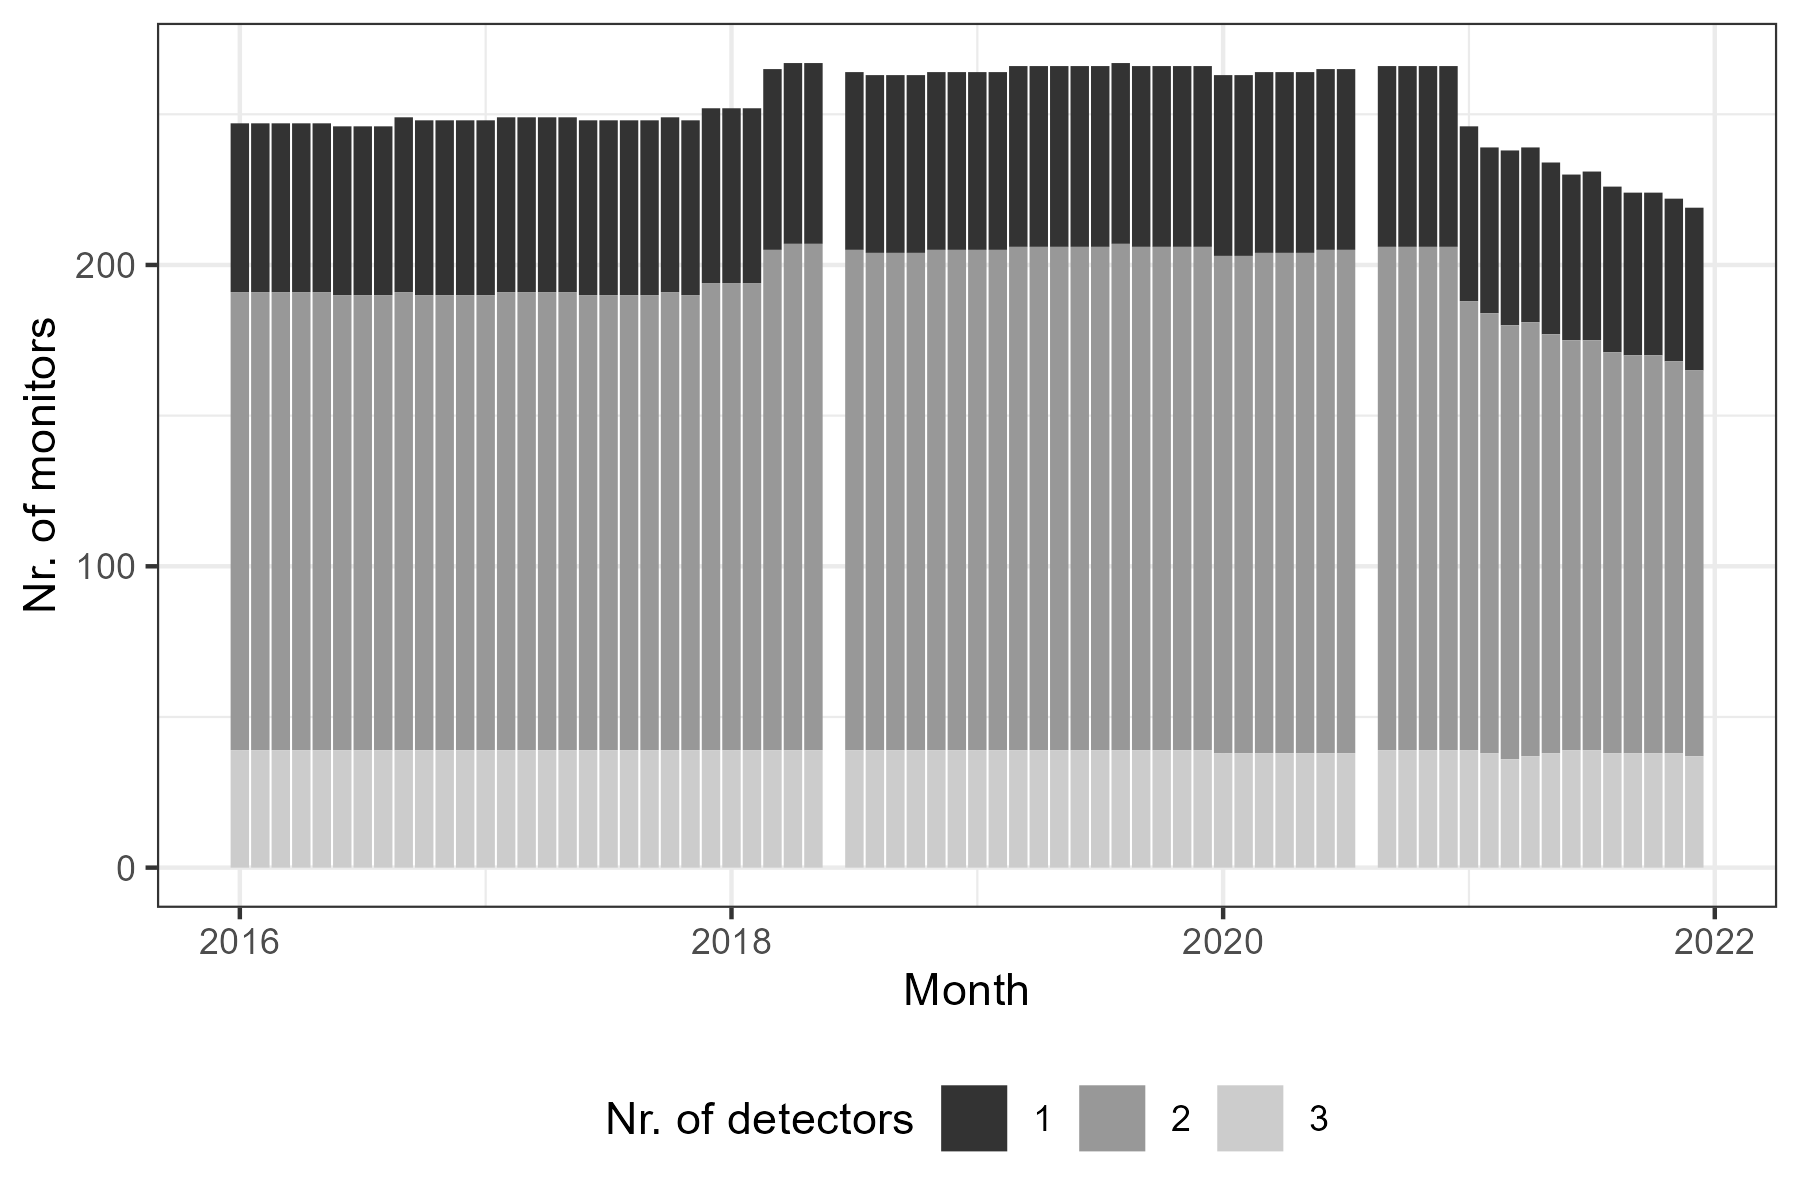
\includegraphics[width = .49\textwidth]{../04_figures/nrmonitors_per_yearmonth.png}
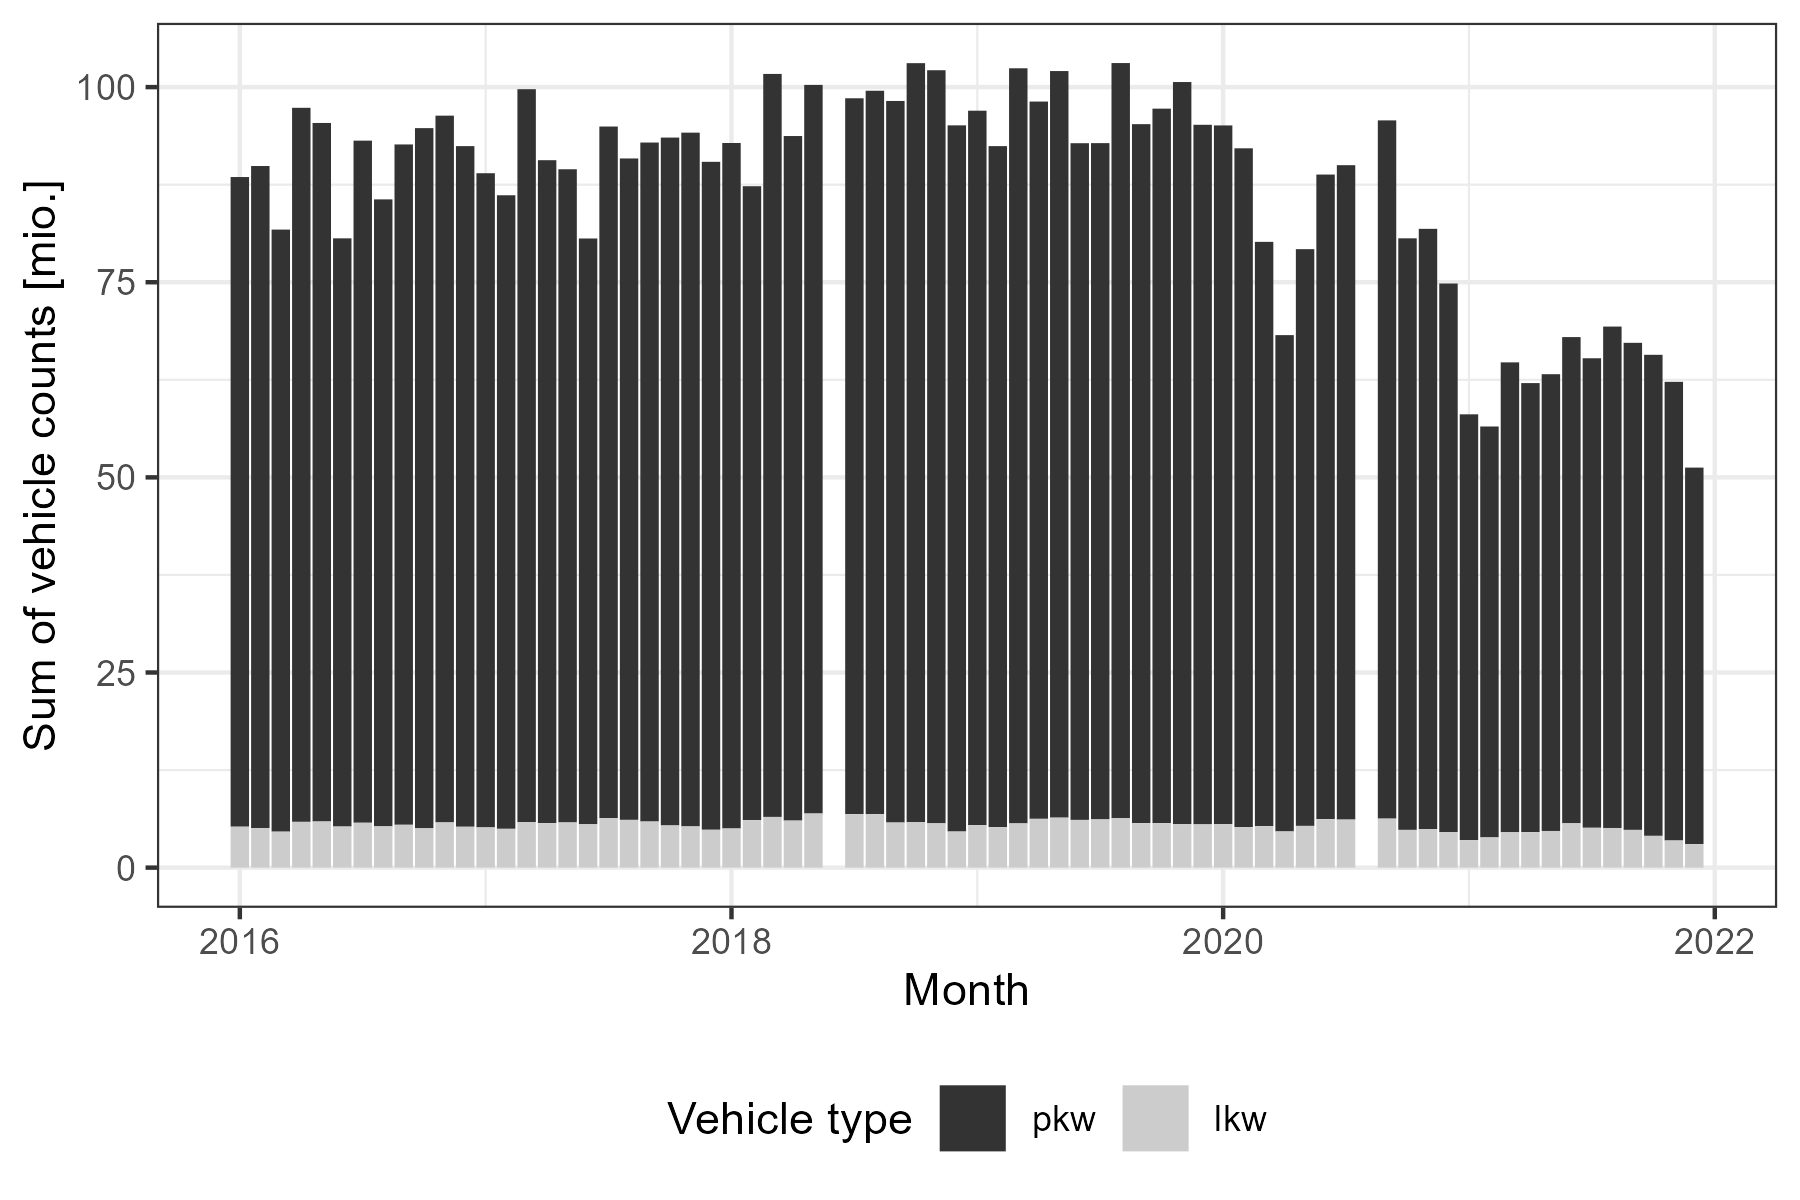
\includegraphics[width = .49\textwidth]{../04_figures/yearmonth_sum.png}
\end{figure}
%
\begin{figure}[!htb]
\centering
\caption{Average hourly vehicle counts and velocity per month}
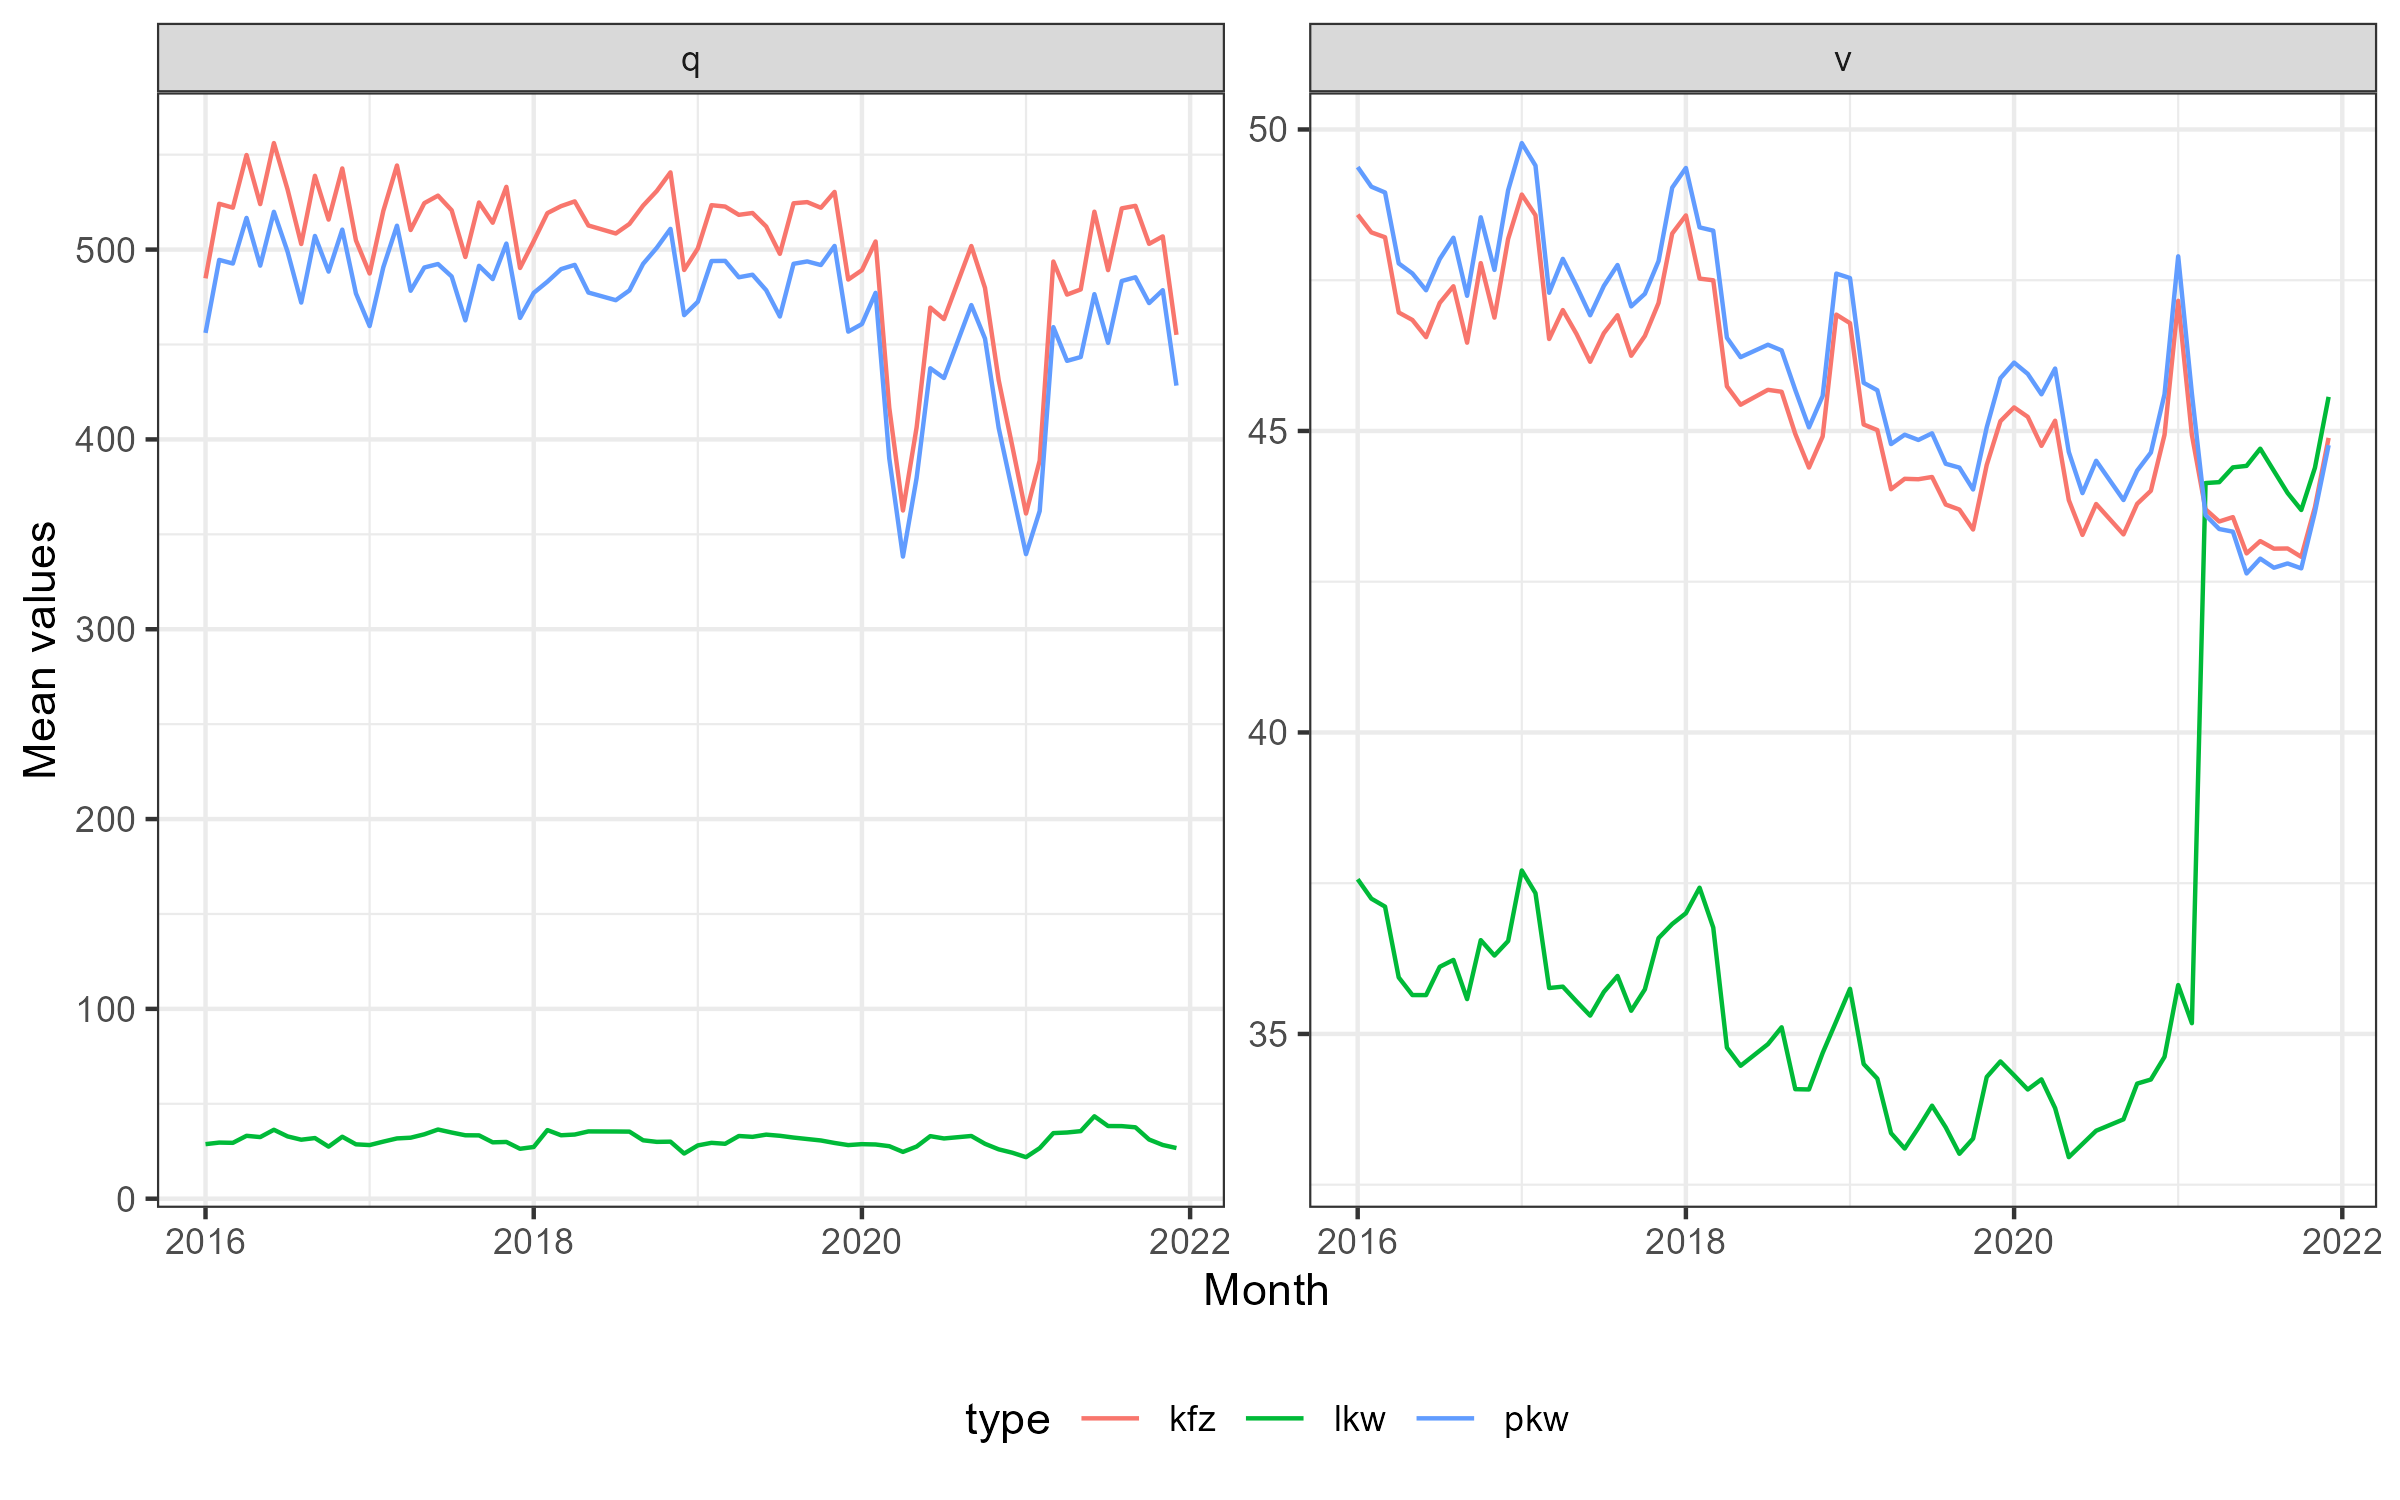
\includegraphics[width = .65\textwidth]{../04_figures/yearmonth_avg.png}
\end{figure}
%
\begin{figure}[!htb]
\centering
\caption{Number of zero-valued hours per month}
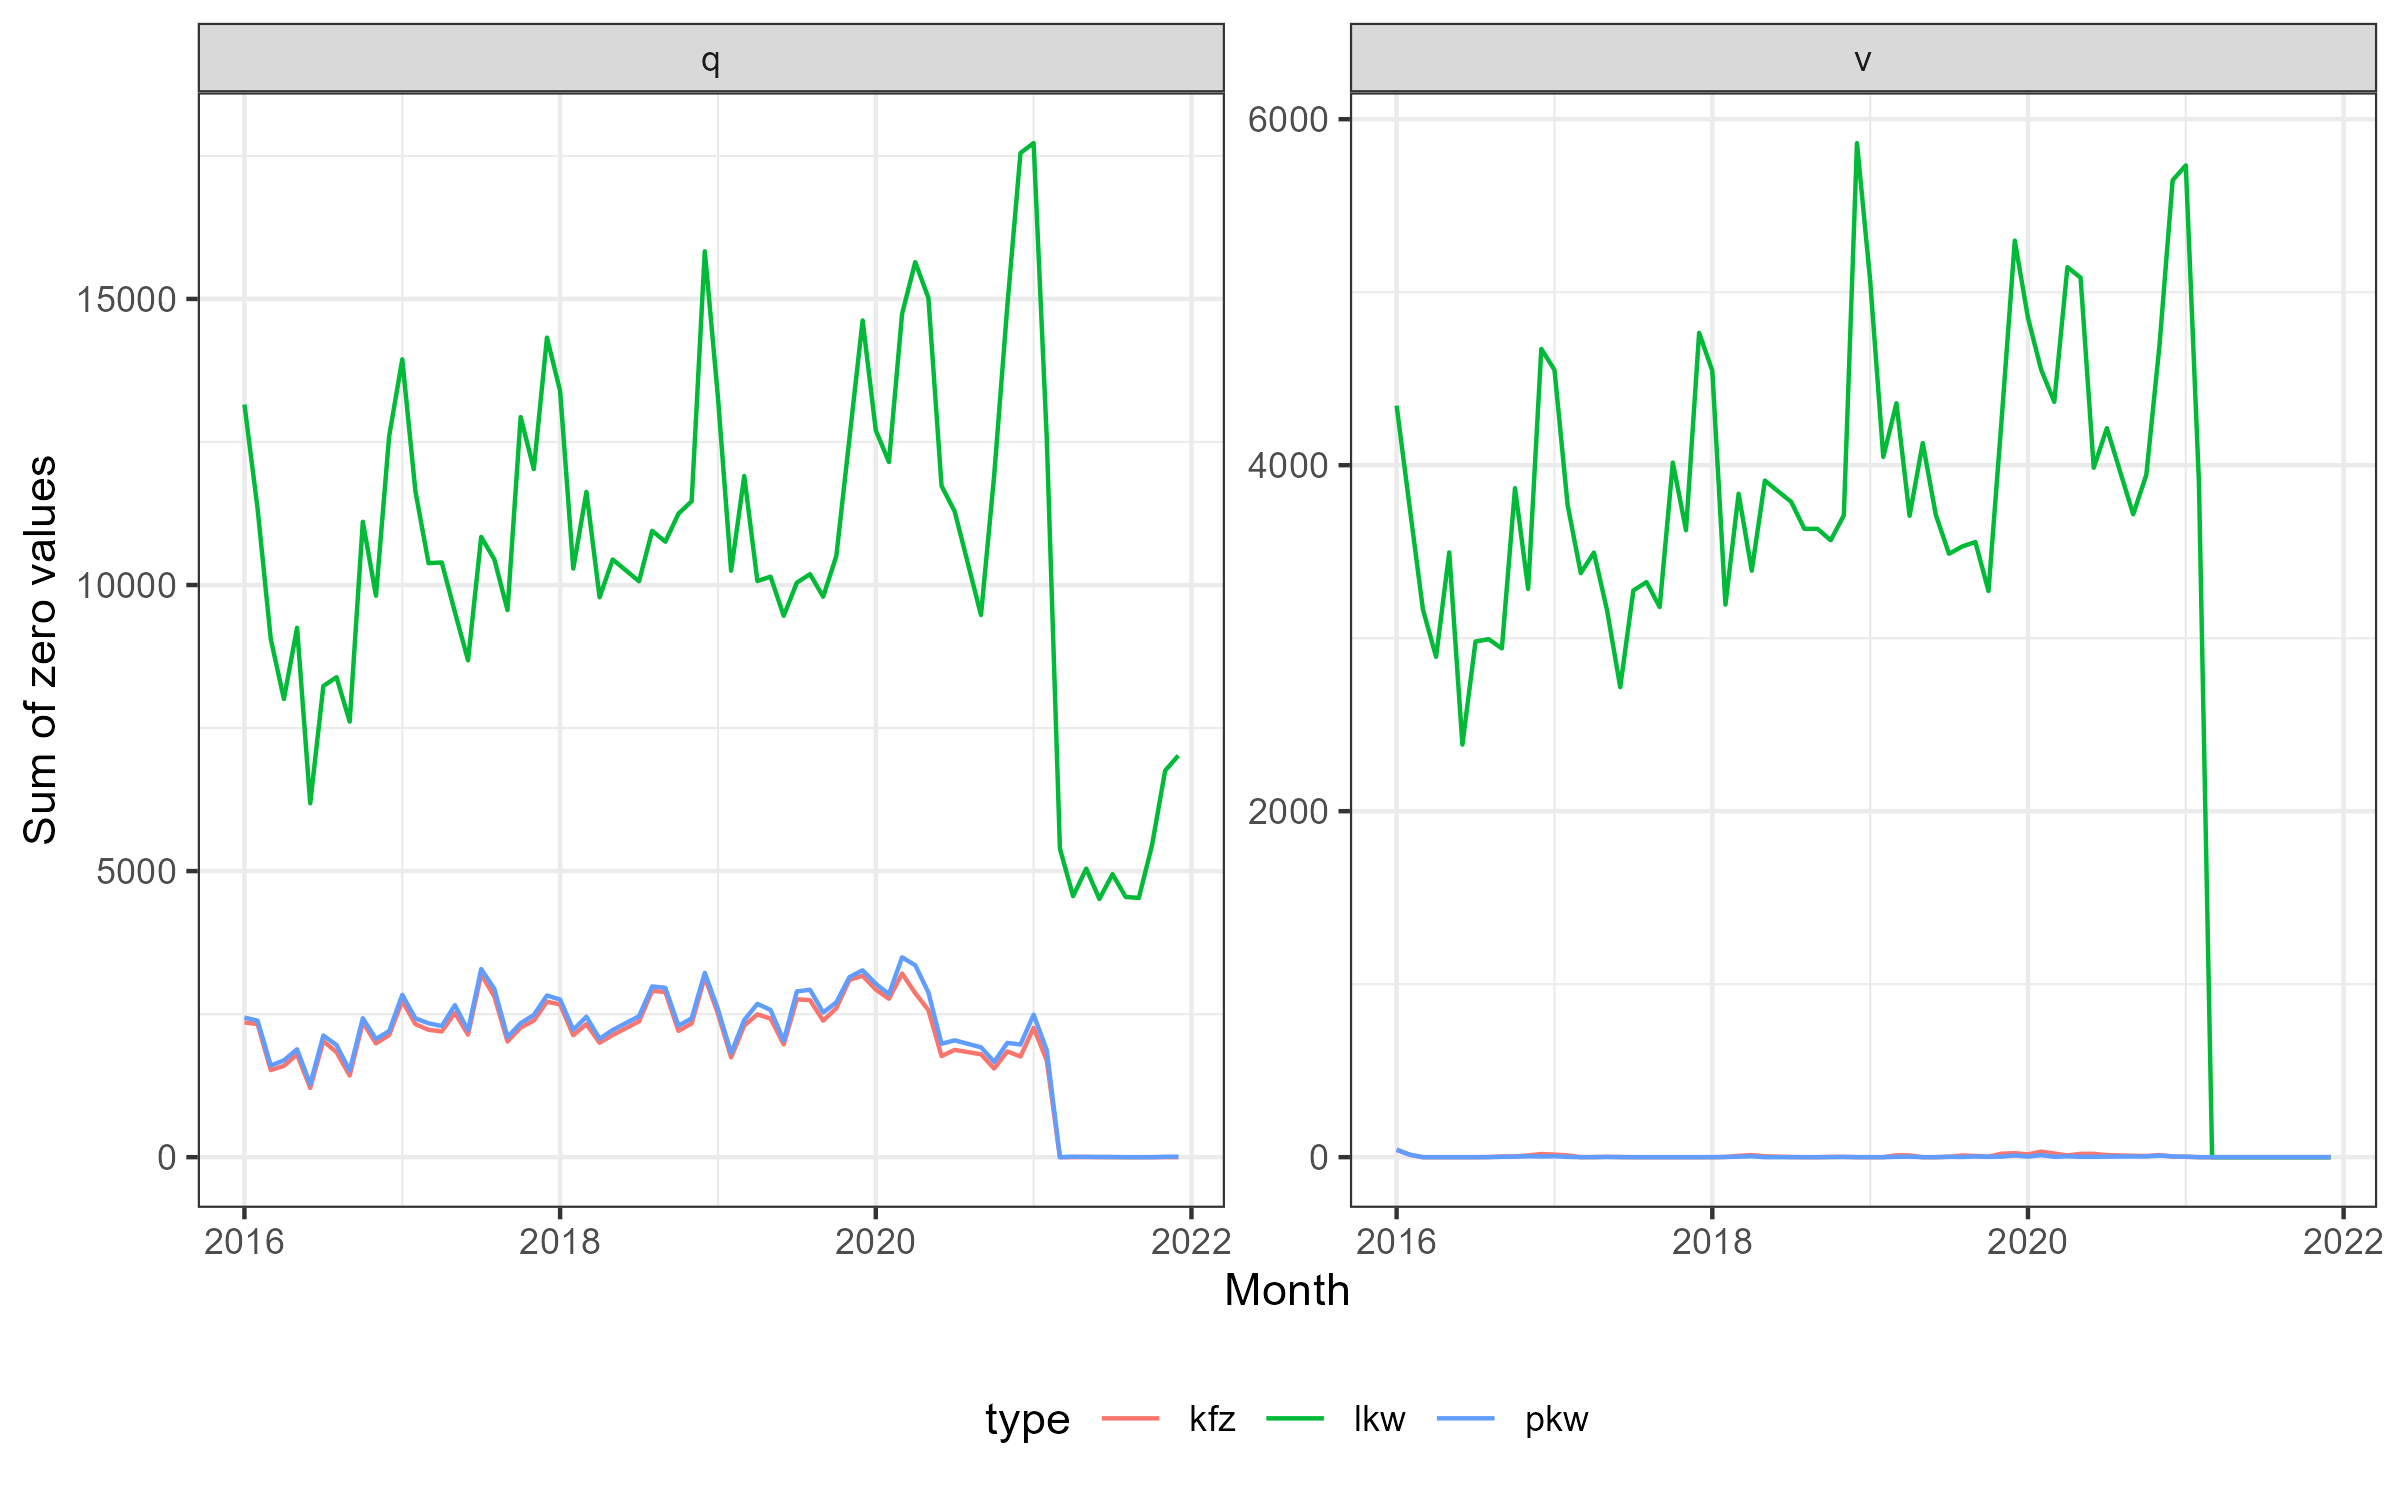
\includegraphics[width = .65\textwidth]{../04_figures/yearmonth_zeros.png}
\end{figure}

\clearpage\FloatBarrier
\subsection{Daily aggregation}

Aggregate hourly to daily $\rightarrow$ Sum counts; average velocities; NA if $<$ 24h of available data

\begin{figure}[!htb]
\centering
\caption{Share of incomplete daily measurements per month}
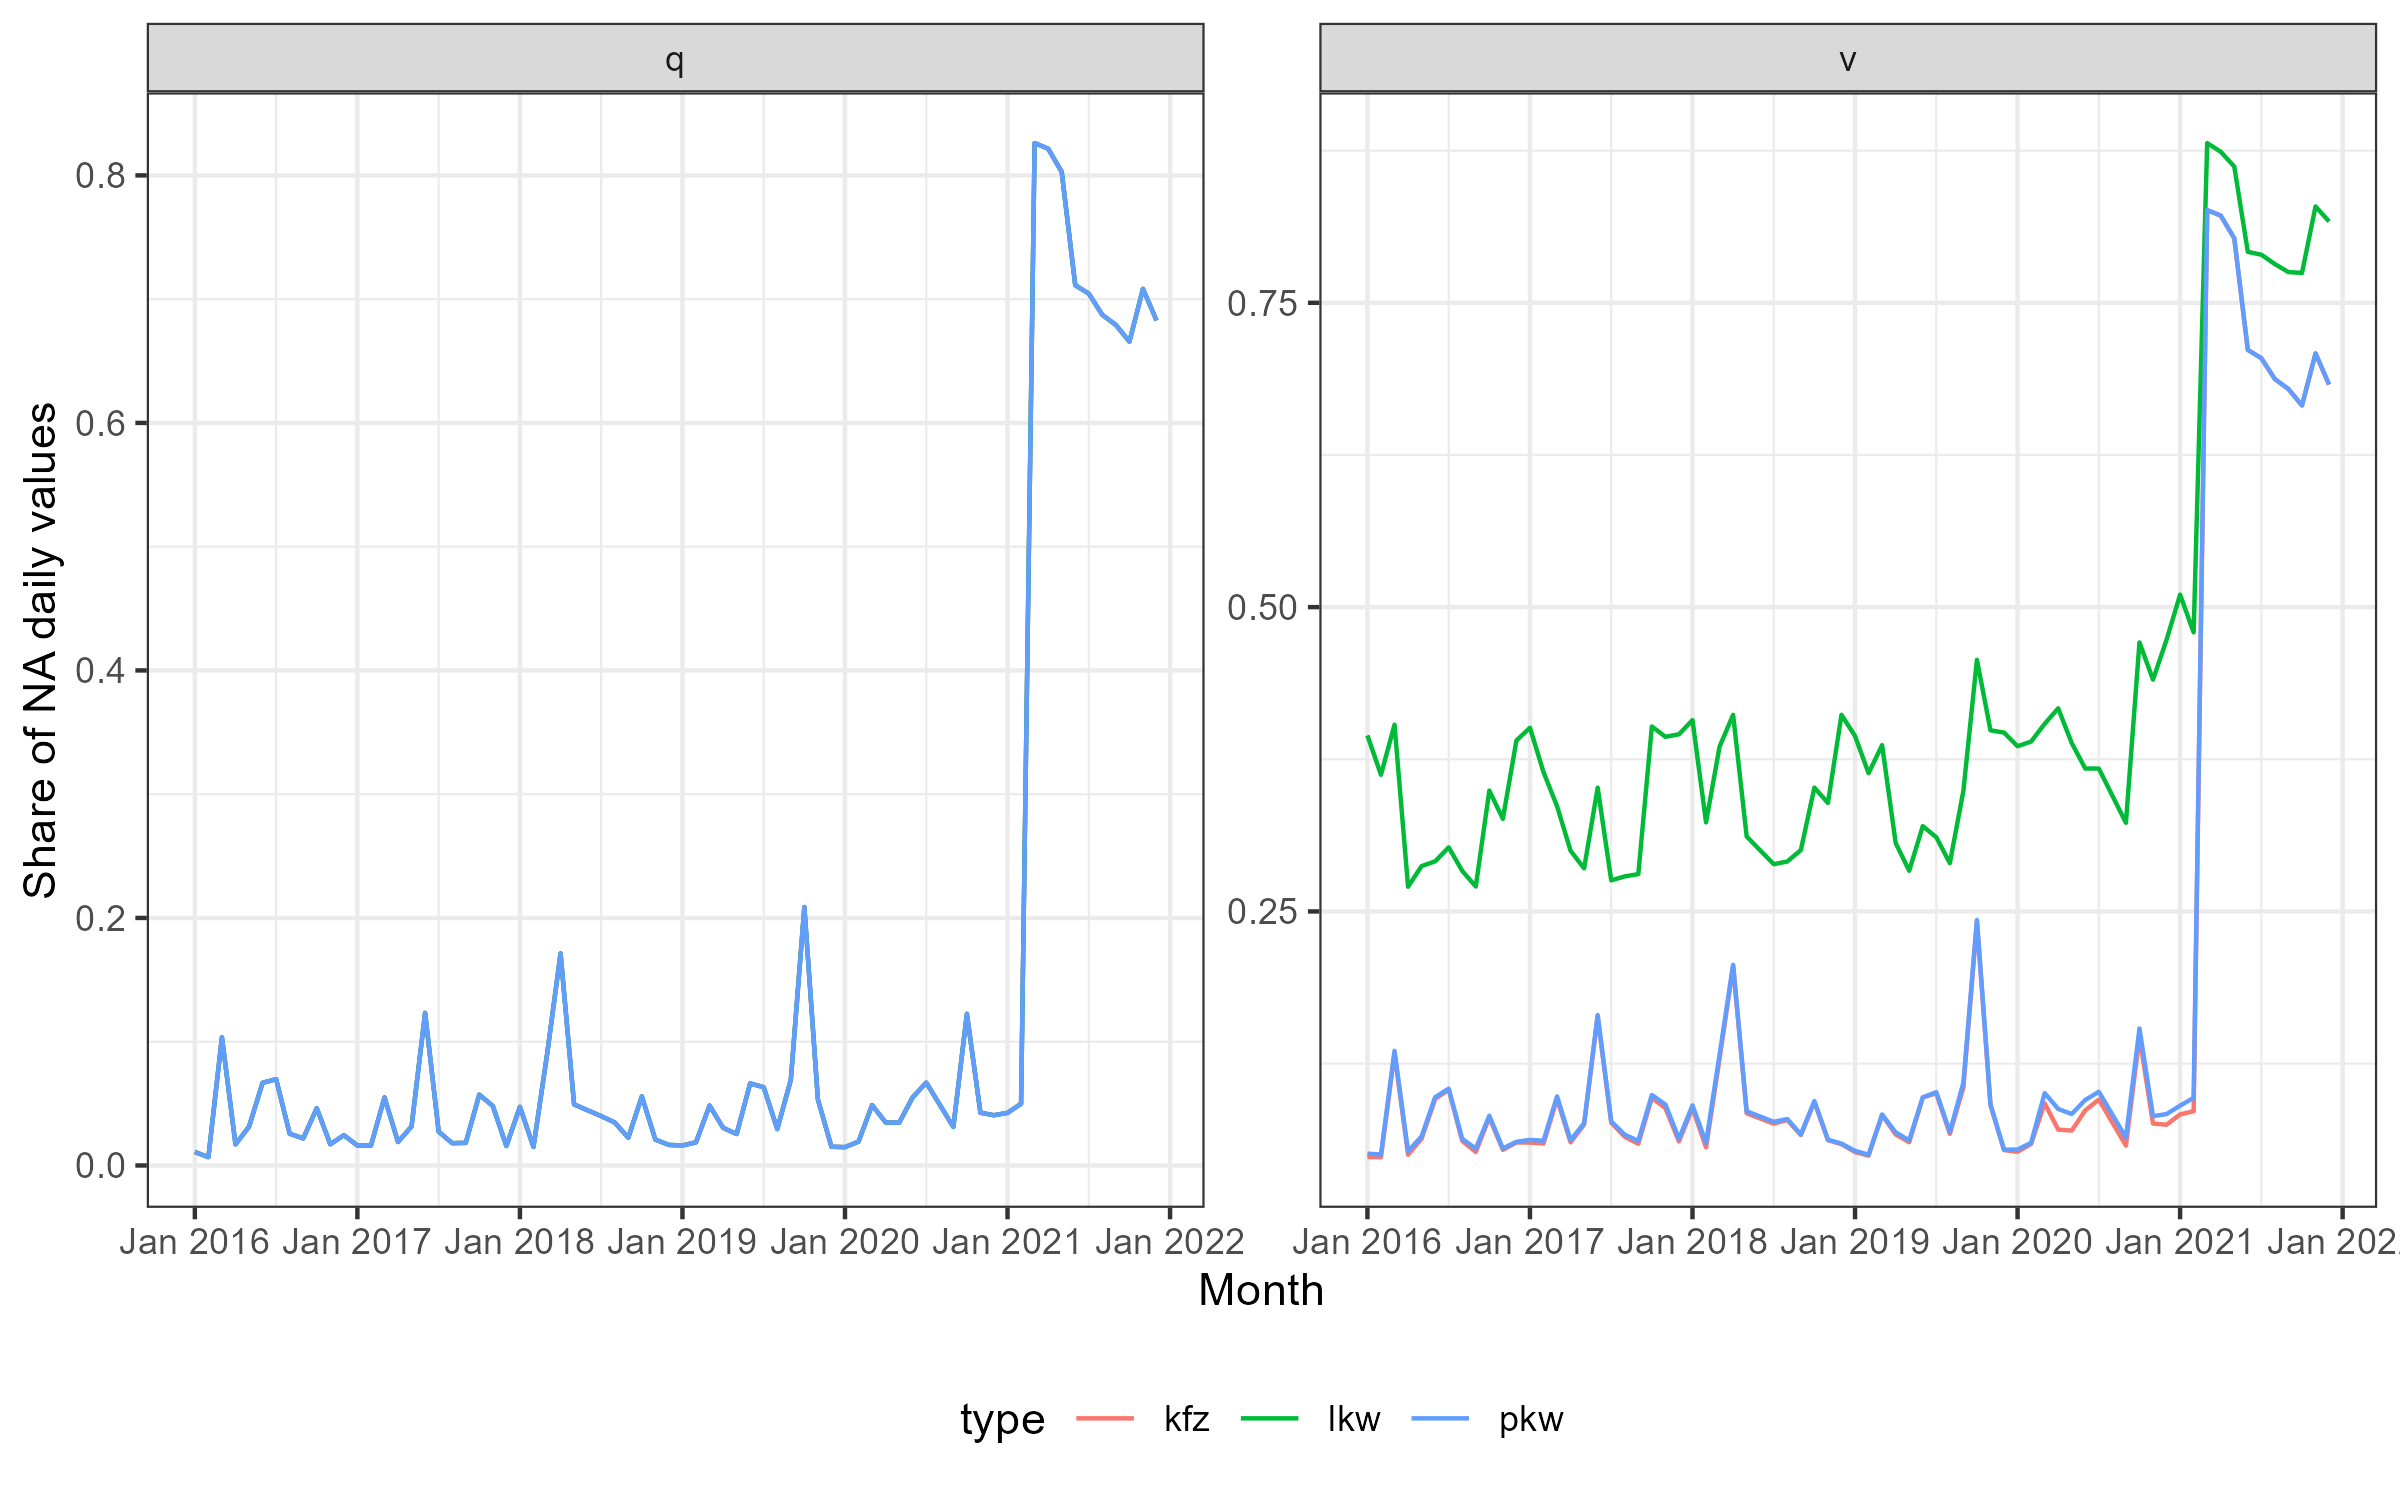
\includegraphics[width = .65\textwidth]{../04_figures/daily_incomplete_share.png}
\end{figure}


%%%%%%%%%%%%%%%%%%%%%%%%%%%%%%%%%%%%%%%%%%%%%%%%%%%%%%%%%%%%%%%%%%%%
\clearpage\FloatBarrier
\section{Data on diesel bans}

\begin{itemize}
	\item List of diesel bans obtained from UBA's website: \url{https://gis.uba.de/website/umweltzonen/index.php#dfv}
	\item Note: Diesel ban in Munich's inner city center since 01.01.2023 (Diesel (außer Lieferverkehr und Anwohner) erst ab Euro 5/VI frei)
\end{itemize}

% latex table generated in R 4.2.2 by xtable 1.8-4 package
% Mon Aug 28 13:10:18 2023
\begin{table}[ht]
\centering
\begingroup\scriptsize
\begin{tabular}{lp{1.55in}p{1in}lll}
  \toprule
bl\_name & name & stringency & start\_date & end\_date & length \\ 
  \midrule
Baden-Württemberg & Stuttgart (Gebiet der Umweltzone Stuttgart) & alle Fahrzeuge mit Dieselmotoren bis Euro 4/IV & 2019-01-01 &  & 0.00 \\ 
  Baden-Württemberg & Stuttgart - Abschnitt "B14 (Am Neckartor)" & Diesel-Pkw bis Euro 5 & 2020-01-01 &  & 327.70 \\ 
  Baden-Württemberg & Stuttgart - Abschnitt "B14 (Hauptstätter Straße)" & Diesel-Pkw bis Euro 5 & 2020-01-01 &  & 703.25 \\ 
  Baden-Württemberg & Stuttgart - Abschnitt "B27 (Charlottenstraße, Hohenheimer Straße, Neue Weinsteige)" & Diesel-Pkw bis Euro 5 & 2020-01-01 &  & 3828.35 \\ 
  Baden-Württemberg & Stuttgart - Abschnitt "B27 (Heilbronner Straße)" & Diesel-Pkw bis Euro 5 & 2020-01-01 &  & 947.61 \\ 
  Baden-Württemberg & Stuttgart (kleine UWZ) & Diesel-Pkw bis Euro 5 & 2020-07-01 &  & 0.00 \\ 
  Berlin & Berlin - Abschnitt "Alt-Moabit" & alle Fahrzeuge mit Dieselmotoren bis Euro 5/V & 2019-11-01 &  & 162.64 \\ 
  Berlin & Berlin - Abschnitt "Hermannstraße" & alle Fahrzeuge mit Dieselmotoren bis Euro 5/V & 2019-11-01 &  & 240.07 \\ 
  Berlin & Berlin - Abschnitt "Leipziger Straße" & alle Fahrzeuge mit Dieselmotoren bis Euro 5/V & 2019-11-01 &  & 822.66 \\ 
  Berlin & Berlin - Abschnitt "Silbersteinstraße" & alle Fahrzeuge mit Dieselmotoren bis Euro 5/V & 2019-11-01 &  & 679.20 \\ 
  Hamburg & Hamburg - Abschnitt "Max-Brauer-Allee" & alle Fahrzeuge mit Dieselmotoren bis Euro 5/V & 2018-05-31 &  & 569.83 \\ 
  Hamburg & Hamburg - Abschnitt "Stresemannstraße" & Diesel-Lkw über 3,5 t bis Euro V & 2018-05-31 &  & 3003.28 \\ 
  Hessen & Darmstadt - Abschnitt "Heinrichstraße" & alle Fahrzeuge mit Dieselmotoren bis Euro 5/V und Pkw mit Ottomotoren bis Euro 2 & 2019-06-01 &  & 667.91 \\ 
  Hessen & Darmstadt - Abschnitt "Hügelstraße" & Diesel-Pkw bis Euro 5 und Pkw mit Ottomotoren bis Euro 2 & 2019-06-01 &  & 307.64 \\ 
  Berlin & Berlin - Abschnitt "Brückenstraße, Jannowitzbrücke" & alle Fahrzeuge mit Dieselmotoren bis Euro 5/V & 2019-11-01 & 2021-06-01 & 470.86 \\ 
  Berlin & Berlin - Abschnitt "Friedrichstraße" & alle Fahrzeuge mit Dieselmotoren bis Euro 5/V & 2019-11-01 & 2021-06-01 & 152.20 \\ 
  Berlin & Berlin - Abschnitt "Reinhardtstraße" & alle Fahrzeuge mit Dieselmotoren bis Euro 5/V & 2019-11-01 & 2021-06-01 & 197.00 \\ 
  Berlin & Berlin - Abschnitt "Stromstraße" & alle Fahrzeuge mit Dieselmotoren bis Euro 5/V & 2019-11-01 & 2021-06-01 & 193.98 \\ 
   \bottomrule
\end{tabular}
\endgroup
\caption{List of diesel bans} 
\end{table}



%%%%%%%%%%%%%%%%%%%%%%%%%%%%%%%%%%%%%%%%%%%%%%%%%%%%%%%%%%%%%%%%%%%%
\section{Weather data}

\begin{itemize}
	\item Daily weather readings from DWD: 
	\begin{itemize}
		\item Temperature (mean, min, max) [\degree C] 
		\item Precipitation [mm]
		\item Sunshine [h]
		\item Relative humidity [\%] 
		\item Wind speed (mean, max) [m/s] 
		\item Atmospheric pressure [hPa]
	\end{itemize}
	\item Interpolate weather at the location of pollution monitors via Inverse Distance Weighting (r = 100km, p = 2)
\end{itemize}

%%%%%%%%%%%%%%%%%%%%%%%%%%%%%%%%%%%%%%%%%%%%%%%%%%%%%%%%%%%%%%%%%%%%
\clearpage\FloatBarrier
\section{Sample selection and descriptives}

\noindent \textbf{Sample selection}
\begin{itemize}
	\item Discard 2021 due to incomplete data (zero values eliminated?) $\rightarrow$ 2016-2020
\end{itemize}

\vspace{0.5cm}
\noindent \textbf{Treatment definition}
\begin{itemize}
	\item Monitor locations within pre-specified distance to diesel ban (preferred 25m, robustness 15m, 75m, 150m)
\end{itemize}

% latex table generated in R 4.2.2 by xtable 1.8-4 package
% Mon Aug 28 16:38:06 2023
\begin{table}[!htb]
\centering
\begingroup\footnotesize
\begin{tabular}{llllll}
  \toprule
& \multicolumn{3}{c}{Inside ban} & Outside ban & Outside $>$ 1500m \\ \cmidrule(r){2-4} \cmidrule(r){5-5} \cmidrule(r){6-6}
variable & Total & Pre & Post & Total1 & Total2 \\ 
  \midrule
Intensity KFZ [thsd. vehicles per day] & 13.359 & 13.886 & 11.641 & 12.068 & 12.143 \\ 
   & (5.517) & (5.594) & (4.900) & (6.410) & (5.711) \\ 
  Intensity PKW [thsd. vehicles per day] & 12.674 & 13.168 & 11.064 & 11.334 & 11.436 \\ 
   & (5.123) & (5.175) & (4.615) & (6.085) & (5.441) \\ 
  Intensity LKW  [thsd. vehicles per day] & 0.685 & 0.718 & 0.577 & 0.743 & 0.708 \\ 
   & (0.501) & (0.527) & (0.387) & (0.908) & (0.675) \\ 
  Speed KFZ [km/h] & 39.632 & 40.313 & 37.407 & 46.288 & 47.059 \\ 
   & (5.525) & (5.599) & (4.646) & (8.946) & (8.998) \\ 
  Speed PKW  [km/h] & 40.078 & 40.770 & 37.818 & 47.039 & 47.728 \\ 
   & (5.620) & (5.688) & (4.756) & (9.084) & (9.102) \\ 
  Speed LKW  [km/h] & 29.868 & 30.340 & 28.276 & 35.527 & 36.342 \\ 
   & (6.872) & (7.234) & (5.193) & (8.951) & (8.863) \\ 
  Dist. to ban [m] & 4.495 & 4.434 & 4.694 & 3541.262 & 4602.644 \\ 
   & (3.159) & (3.137) & (3.236) & (2817.742) & (2673.737) \\ 
  Rain [mm] & 1.464 & 1.523 & 1.273 & 1.472 & 1.471 \\ 
   & (1.079) & (1.181) & (0.605) & (1.081) & (1.082) \\ 
  Temperature [C] & 10.810 & 11.113 & 9.823 & 10.721 & 10.718 \\ 
   & (6.783) & (7.145) & (5.344) & (6.739) & (6.734) \\ 
  Sunshine [h] & 4.978 & 5.137 & 4.458 & 5.038 & 5.056 \\ 
   & (2.989) & (2.967) & (3.012) & (2.992) & (2.996) \\ 
  Wind speed [m/s] & 3.621 & 3.629 & 3.596 & 3.659 & 3.672 \\ 
   & (0.508) & (0.486) & (0.575) & (0.537) & (0.545) \\ 
  Humidity [\%] & 72.819 & 72.316 & 74.463 & 73.548 & 73.642 \\ 
   & (10.352) & (9.979) & (11.378) & (10.256) & (10.260) \\ 
\midrule N.Observations & 499&382&117&14437&10292\\
 N.Units & 9&9&9&258&185\\
   \bottomrule
\end{tabular}
\endgroup
\caption{Descriptives on traffic and weather for treated and control samples (monthly avg.)} 
\end{table}

%
%% latex table generated in R 4.2.2 by xtable 1.8-4 package
% Mon Aug 28 16:38:11 2023
\begin{table}[!htb]
\centering
\begingroup\footnotesize
\begin{tabular}{lrrrrrrrr}
  \toprule
pol & t15\_pre & t15\_post & t25\_pre & t25\_post & t75\_pre & t75\_post & t150\_pre & t150\_post \\ 
  \midrule
q\_kfz\_N & 9 & 9 & 9 & 9 & 10 & 10 & 13 & 13 \\ 
  q\_kfz\_nobs & 11118 & 3391 & 11118 & 3391 & 11757 & 3772 & 15693 & 4920 \\ 
  q\_pkw\_N & 9 & 9 & 9 & 9 & 10 & 10 & 13 & 13 \\ 
  q\_pkw\_nobs & 11118 & 3391 & 11118 & 3391 & 11757 & 3772 & 15693 & 4920 \\ 
  q\_lkw\_N & 9 & 9 & 9 & 9 & 10 & 10 & 13 & 13 \\ 
  q\_lkw\_nobs & 11118 & 3391 & 11118 & 3391 & 11757 & 3772 & 15693 & 4920 \\ 
   \bottomrule
\end{tabular}
\endgroup
\caption{Number of treated monitors and complete daily averages} 
\end{table}

%% latex table generated in R 4.2.2 by xtable 1.8-4 package
% Mon Aug 28 16:38:11 2023
\begin{table}[!htb]
\centering
\begingroup\footnotesize
\begin{tabular}{lrrrrrrrr}
  \toprule
pol & t15\_pre & t15\_post & t25\_pre & t25\_post & t75\_pre & t75\_post & t150\_pre & t150\_post \\ 
  \midrule
q\_kfz\_N & 9 & 9 & 9 & 9 & 10 & 10 & 13 & 13 \\ 
  q\_kfz\_nobs & 382 & 117 & 382 & 117 & 404 & 130 & 539 & 169 \\ 
  q\_pkw\_N & 9 & 9 & 9 & 9 & 10 & 10 & 13 & 13 \\ 
  q\_pkw\_nobs & 382 & 117 & 382 & 117 & 404 & 130 & 539 & 169 \\ 
  q\_lkw\_N & 9 & 9 & 9 & 9 & 10 & 10 & 13 & 13 \\ 
  q\_lkw\_nobs & 382 & 117 & 382 & 117 & 404 & 130 & 539 & 169 \\ 
   \bottomrule
\end{tabular}
\endgroup
\caption{Number of treated monitors and monthly averages} 
\end{table}


\begin{figure}[H]
\centering
\caption{Monthly average traffic intensity at monitor locations inside vs. outside bans}
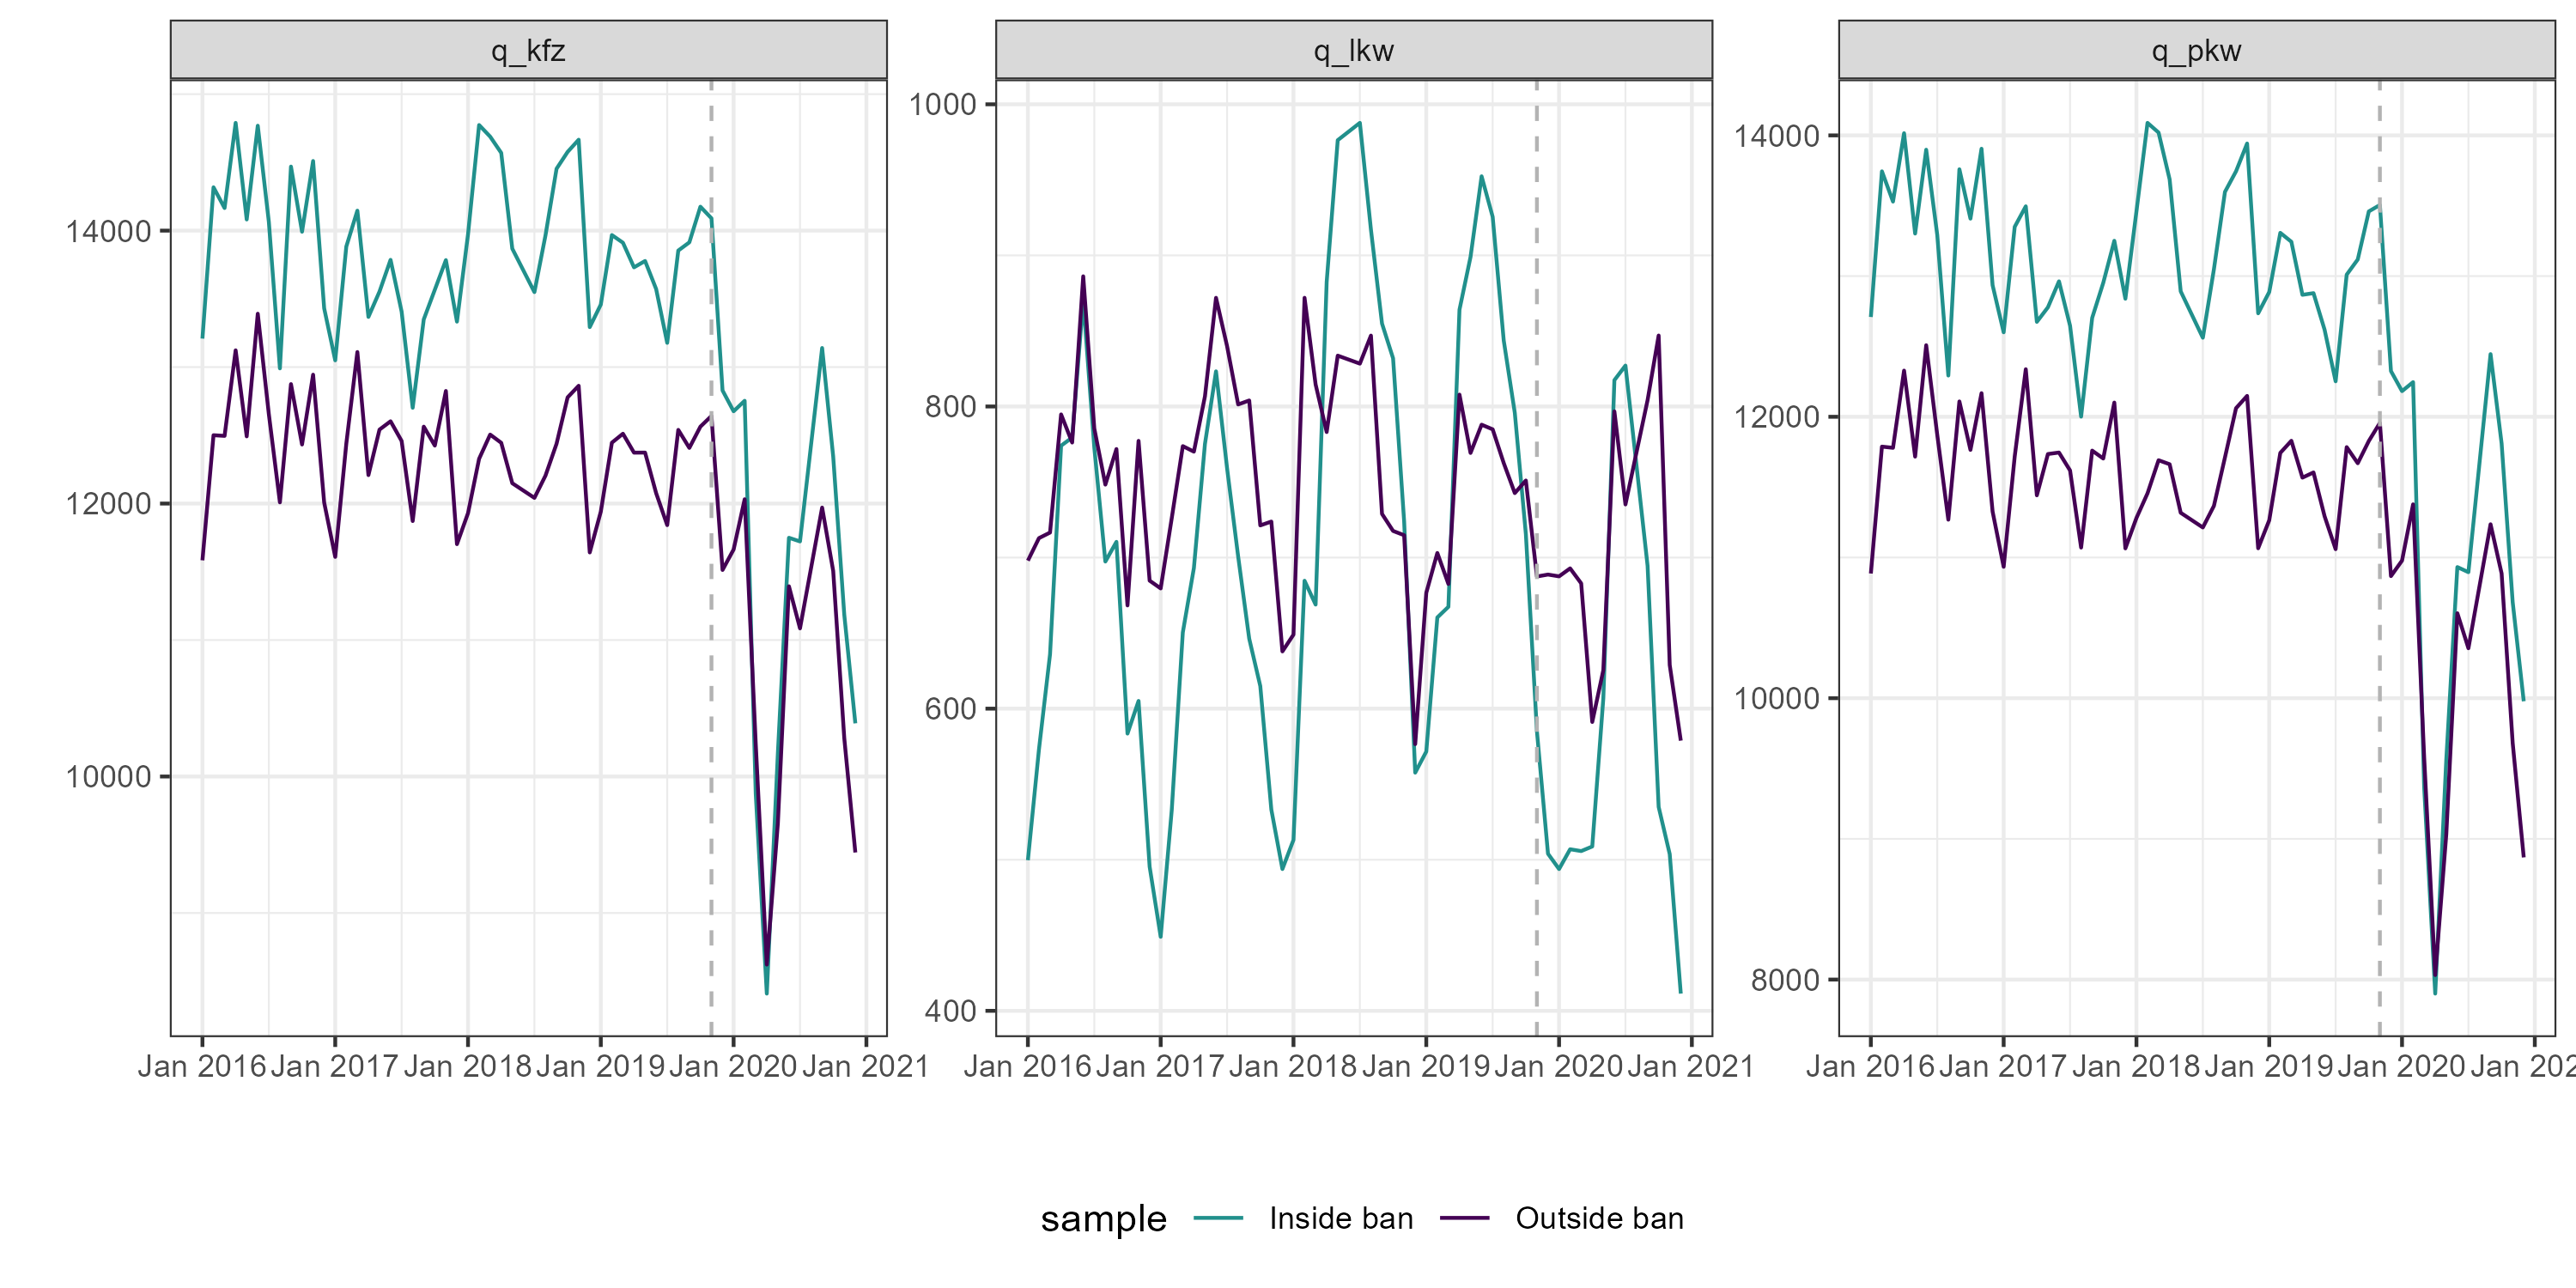
\includegraphics[width = \textwidth]{../04_figures/monthly_unrestricted.png} 
\end{figure}
%%
%\begin{figure}[H]
%\centering
%\caption{Monthly average traffic intensity (centered) for treatment groups and controls ($>$1000m) in the same city}
%\label{fig:geographic_centered}
%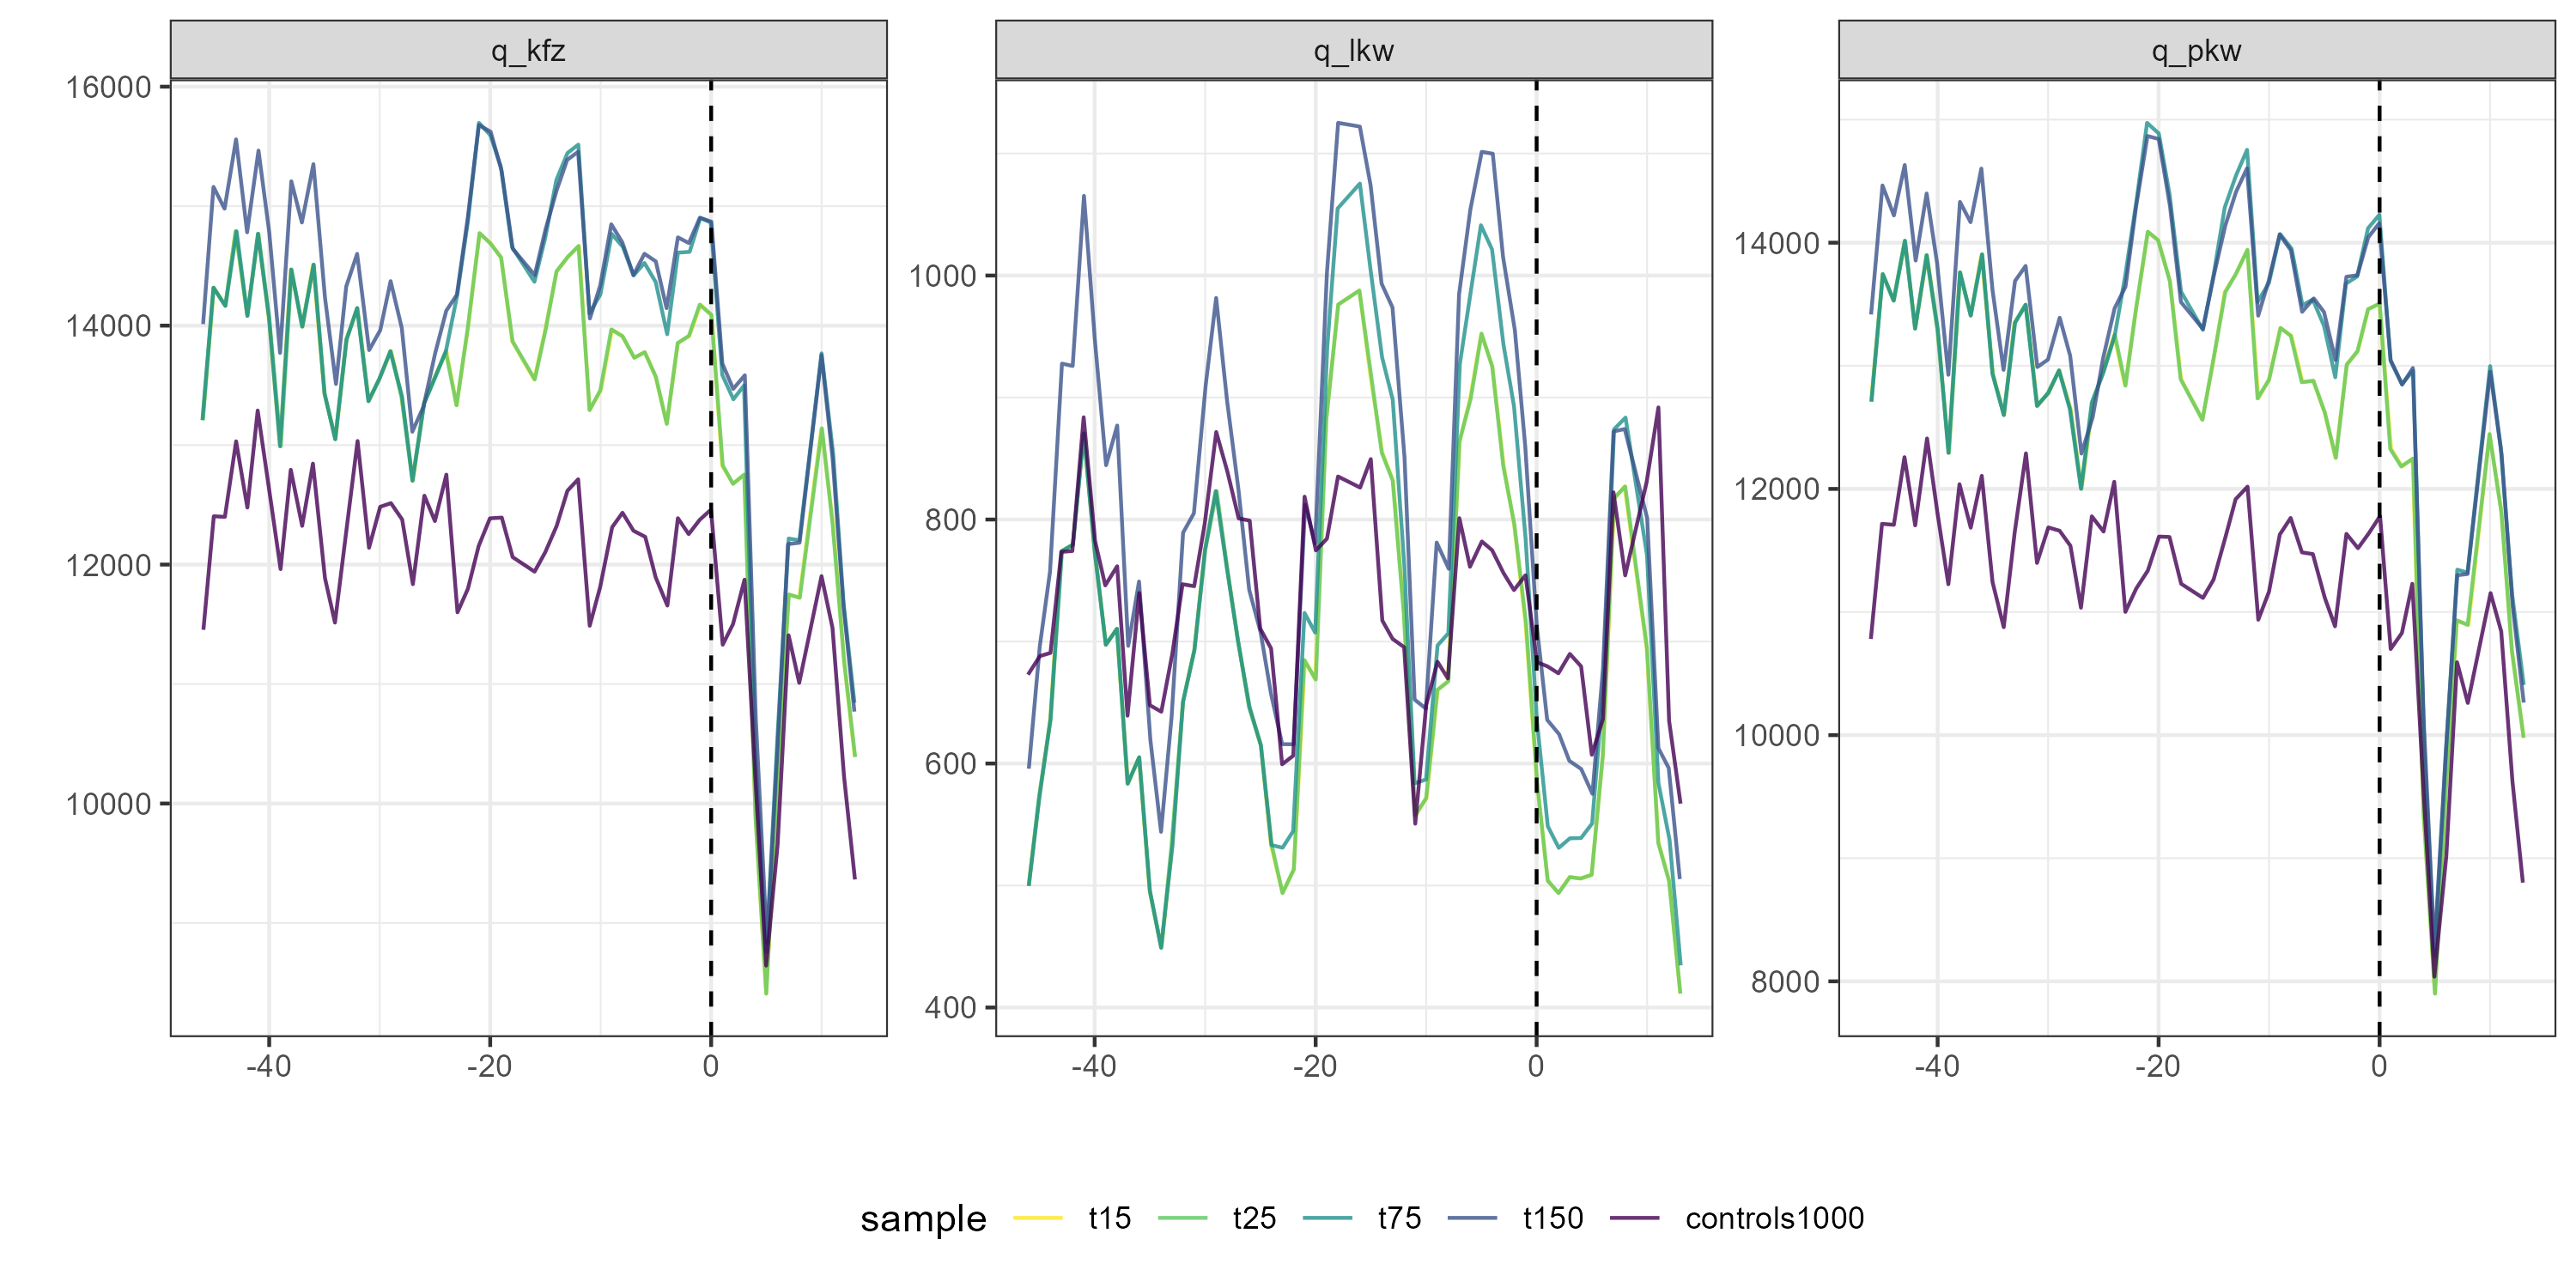
\includegraphics[width = \textwidth]{../04_figures/monthly_cities_centered.png} 
%\end{figure}

%%%%%%%%%%%%%%%%%%%%%%%%%%%%%%%%%%%%%%%%%%%%%%%%%%%%%%%%%%%%%%%%%%%%
\clearpage
\section{Empirical model and results}

Two-way fixed effect model

\begin{equation}
Y_{it} = \beta D_{it} + W_{it}'\gamma + \lambda_i + \tau_t + \epsilon_{it}
\end{equation}

\begin{itemize}
	\item $Y_{it}$ - Average daily (log) vehicle count at location $i$ in month $t$
	\item $D_{it}$ - Treatment indicator equal to 1 after ban implementation
	\item $W_{it}'$ - Average weather at location $i$ in month $t$ (temperature, rain, sunshine, windspeed, rel. humidity)
	\item $\lambda_i$ - Monitor-location fixed effects
	\item $\tau_t$ - Month fixed effects
\end{itemize}


\begin{table}[h]
\caption{Impact of diesel bans on traffic intensity}
\begin{center}
\begin{footnotesize}
\begin{threeparttable}
\begin{tabular}{l c c c c c c c c c}
\toprule
& \multicolumn{3}{c}{KFZ} & \multicolumn{3}{c}{PKW}  & \multicolumn{3}{c}{LKW} \\ \cmidrule(r){2-4} \cmidrule(r){5-7} \cmidrule(r){8-10}
 & (1) & (2) & (3) & (1) & (2) & (3) & (1) & (2) & (3) \\
\midrule
Post   & $-1250^{**}$ & $-1219^{*}$ & $-1213^{*}$ & $-1135^{**}$ & $-1112^{*}$ & $-1096^{*}$ & $-155^{*}$ & $-153^{*}$ & $-170^{*}$ \\
       & $(472)$      & $(476)$     & $(480)$     & $(434)$      & $(437)$     & $(444)$     & $(72)$     & $(75)$     & $(77)$     \\
\midrule
Monitor FEs   & Yes & Yes & Yes  & Yes & Yes & Yes & Yes & Yes & Yes    \\
Year-month FEs     & Yes & Yes & Yes  & Yes & Yes & Yes & Yes & Yes & Yes  \\
Weather     & No & Quadr. & Quint.  & No & Quadr. & Quint. & No & Quadr. & Quint.   \\ \midrule
Nobs   & $12767$      & $12767$     & $12767$     & $12767$      & $12767$     & $12767$     & $12767$    & $12767$    & $12767$    \\
N      & $229$        & $229$       & $229$       & $229$        & $229$       & $229$       & $229$      & $229$      & $229$      \\
Adj.R2 & $1$          & $1$         & $1$         & $1$          & $1$         & $1$         & $0$        & $0$        & $0$        \\
\bottomrule
\end{tabular}
\begin{tablenotes}[flushleft]
\tiny{\item Treated monitors within 25m distance to a diesel ban. 
       Control monitors in cities with diesel ban further away than 1000m from the ban. 
       Standard errors clustered at the monitor level.
       Significance levels $^{***}p<0.001$; $^{**}p<0.01$; $^{*}p<0.05$.}
\end{tablenotes}
\end{threeparttable}
\end{footnotesize}
\label{table:coefficients}
\end{center}
\end{table}

%

\begin{table}[h]
\caption{Impact of diesel bans on traffic intensity (log)}
\begin{center}
\begin{footnotesize}
\begin{threeparttable}
\begin{tabular}{l c c c c c c c c c}
\toprule
& \multicolumn{3}{c}{Log KFZ } & \multicolumn{3}{c}{Log PKW }  & \multicolumn{3}{c}{Log LKW } \\ \cmidrule(r){2-4} \cmidrule(r){5-7} \cmidrule(r){8-10}
 & (1) & (2) & (3) & (1) & (2) & (3) & (1) & (2) & (3) \\
\midrule
Post   & $-0.102^{*}$ & $-0.096$  & $-0.095$  & $-0.095$  & $-0.090$  & $-0.088$  & $-0.163^{*}$ & $-0.156^{*}$ & $-0.161^{*}$ \\
       & $(0.051)$    & $(0.051)$ & $(0.051)$ & $(0.052)$ & $(0.053)$ & $(0.053)$ & $(0.063)$    & $(0.063)$    & $(0.064)$    \\
\midrule
Monitor FEs   & Yes & Yes & Yes  & Yes & Yes & Yes & Yes & Yes & Yes    \\
Year-month FEs     & Yes & Yes & Yes  & Yes & Yes & Yes & Yes & Yes & Yes  \\
Weather     & No & Quadr. & Quint.  & No & Quadr. & Quint. & No & Quadr. & Quint.   \\ \midrule
Nobs   & $12767$      & $12767$   & $12767$   & $12767$   & $12767$   & $12767$   & $12767$      & $12767$      & $12767$      \\
N      & $229$        & $229$     & $229$     & $229$     & $229$     & $229$     & $229$        & $229$        & $229$        \\
Adj.R2 & $0.887$      & $0.887$   & $0.887$   & $0.888$   & $0.888$   & $0.888$   & $0.799$      & $0.800$      & $0.799$      \\
\bottomrule
\end{tabular}
\begin{tablenotes}[flushleft]
\tiny{\item Treated monitors within 25m distance to a diesel ban. 
       Control monitors in cities with diesel ban further away than 1000m from the ban. 
       Standard errors clustered at the monitor level.
       Significance levels $^{***}p<0.001$; $^{**}p<0.01$; $^{*}p<0.05$.}
\end{tablenotes}
\end{threeparttable}
\end{footnotesize}
\label{table:coefficients}
\end{center}
\end{table}

%
%\input{../05_tables/twfe_monthlybinary_bancities_treat25_b1000.tex}
%
\begin{figure}[H]
\centering
\caption{Impact of diesel bans on traffic intensity across different treatment and buffer distances}
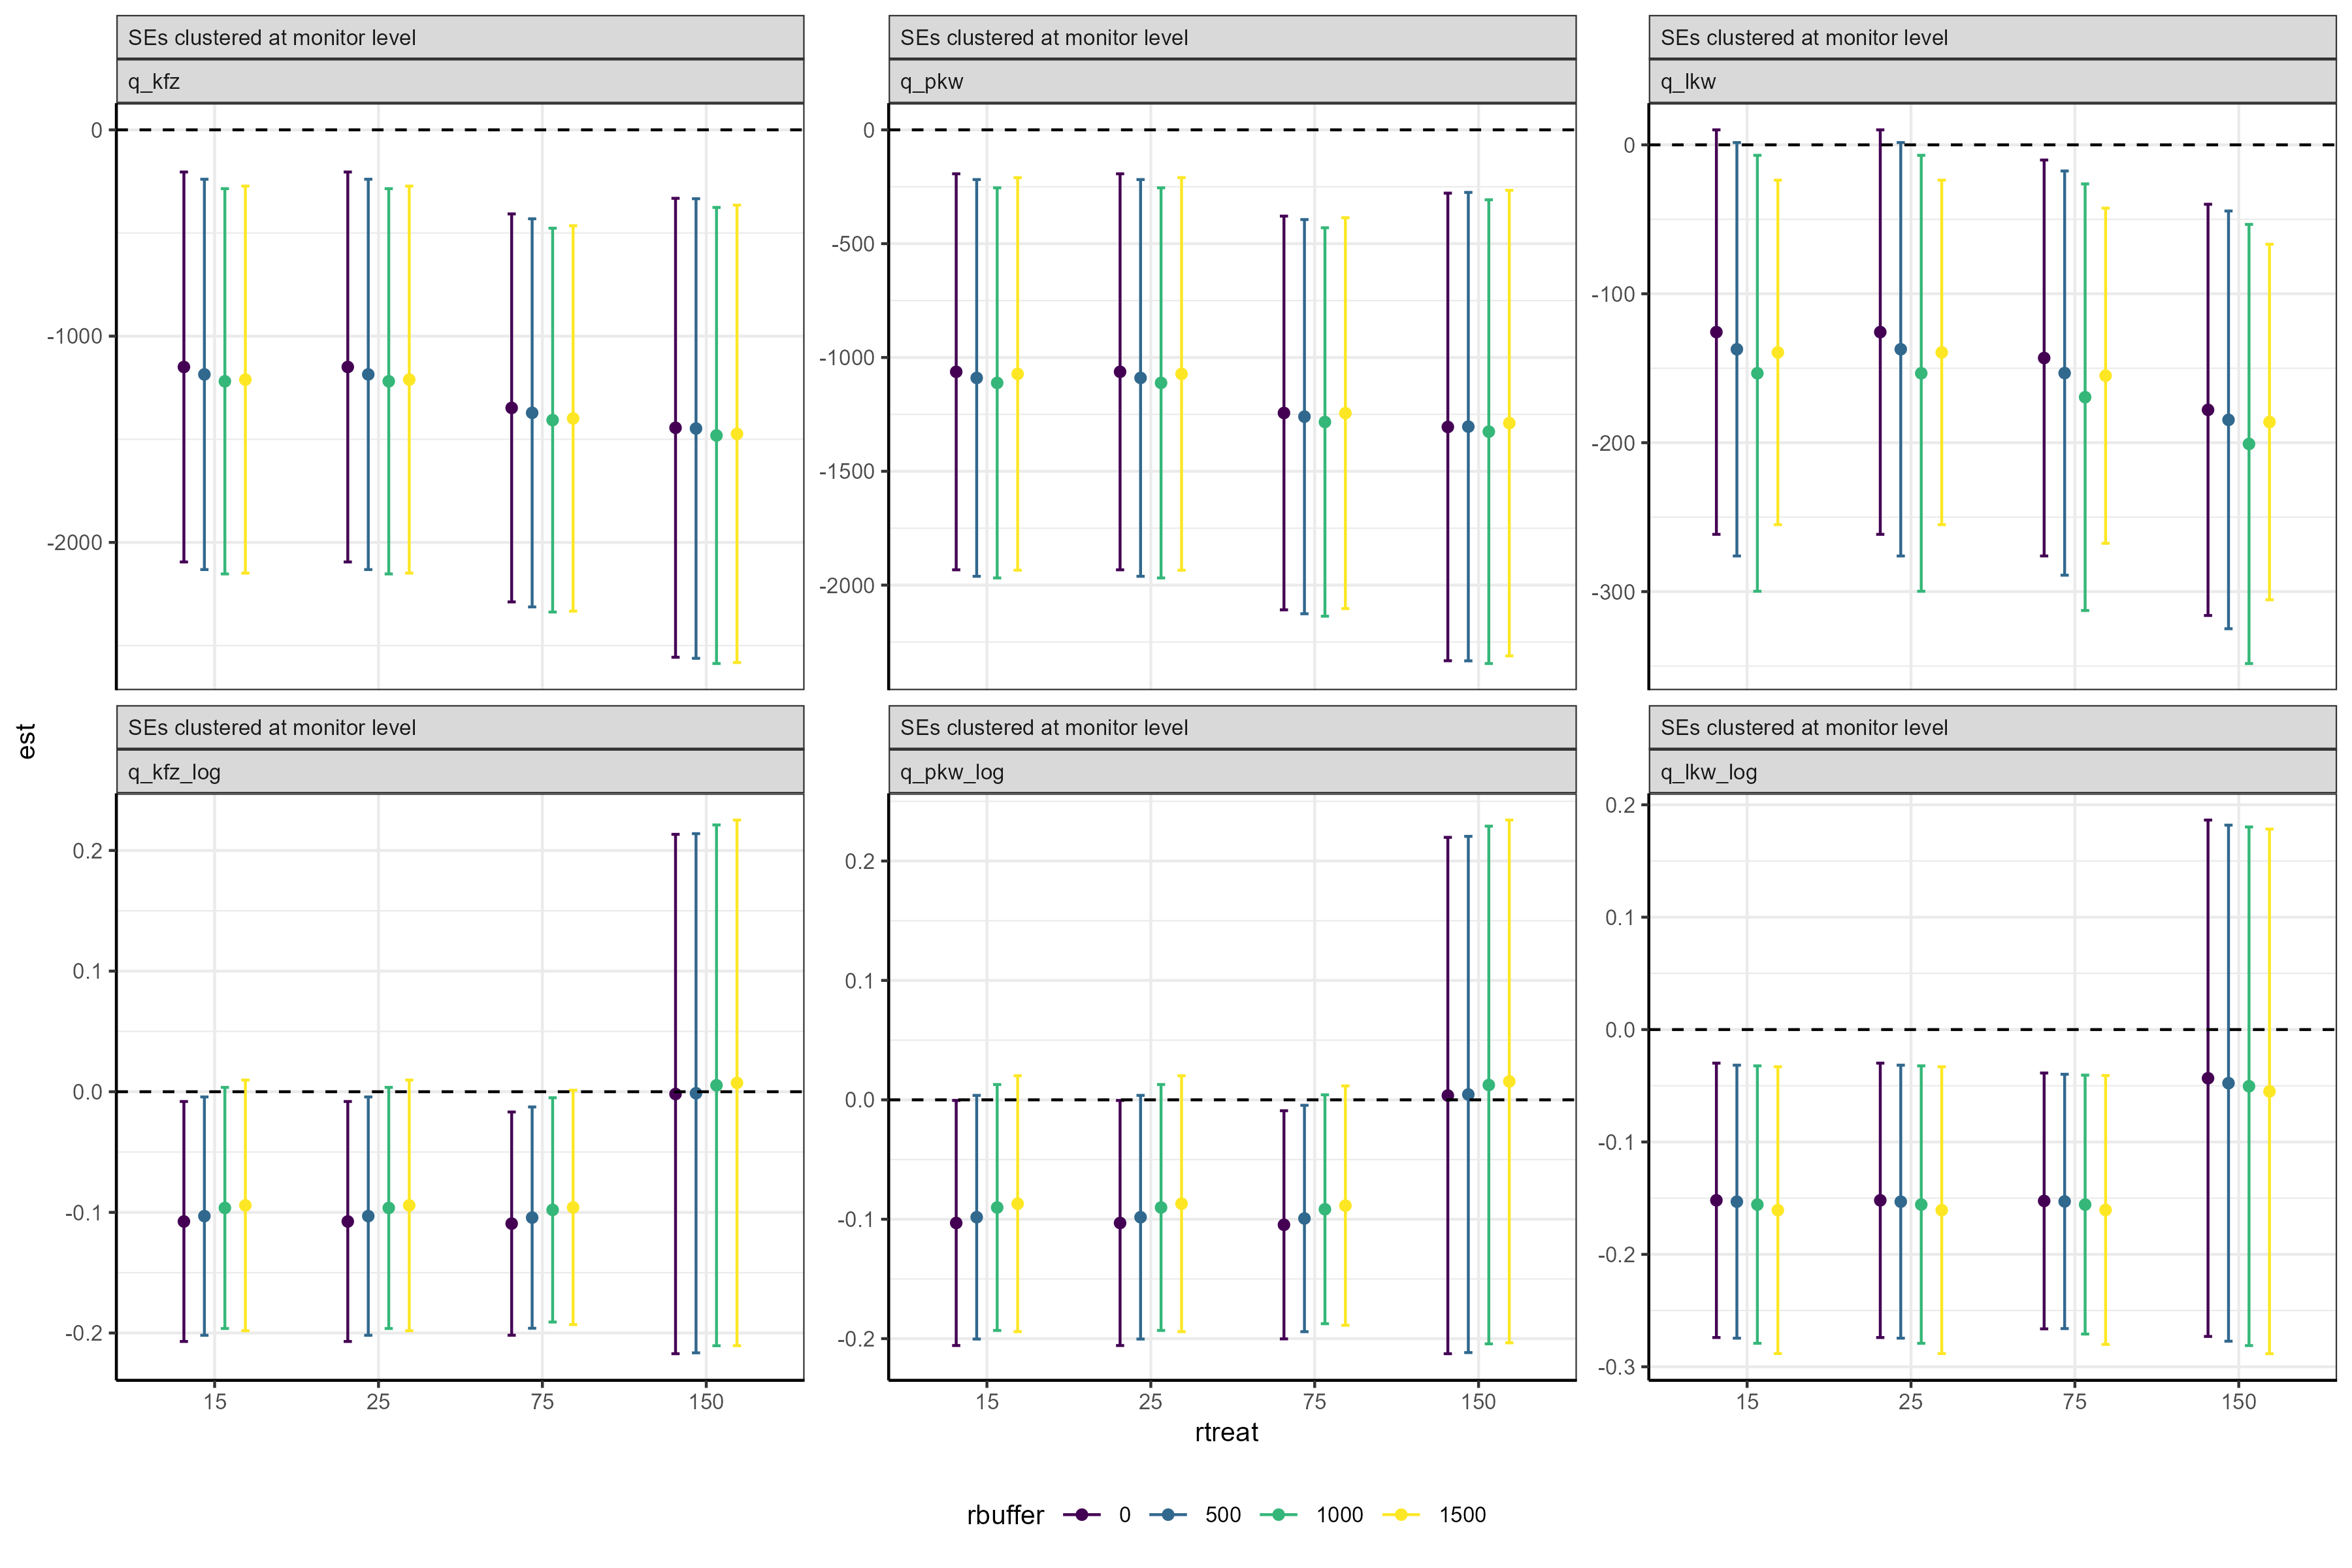
\includegraphics[width = \textwidth]{../04_figures/twfe_monthly_bancities_treatrad_bufferrad.png} 
\notes{rtreat - treatment radius; rbuffer - buffer radius; controls for temp., rain, sunshine, windspeed, rel. humidity with second order polynomials; monitor and year-month FEs; 95\% CIs}
\end{figure}


\begin{table}[h]
\caption{Weather robustness: Impact of diesel bans on KFZ intensity}
\begin{center}
\begin{footnotesize}
\begin{threeparttable}
\begin{tabular}{l c c c c c c c c}
\toprule
& \multicolumn{4}{c}{KFZ} & \multicolumn{4}{c}{Log KFZ}  \\ \cmidrule(r){2-5} \cmidrule(r){6-9}
 & (1) & (2) & (3) & (4) & (1) & (2) & (3) & (4) \\
\midrule
Post   & $-1194.456^{*}$ & $-1182.903^{*}$ & $-1172.883^{*}$ & $-1213.492^{*}$ & $-0.092$  & $-0.090$  & $-0.085$  & $-0.096$  \\
       & $(479.890)$     & $(484.738)$     & $(477.510)$     & $(472.658)$     & $(0.052)$ & $(0.052)$ & $(0.054)$ & $(0.051)$ \\
\midrule
Monitor FEs   & Yes & Yes & Yes  & Yes & Yes & Yes & Yes & Yes     \\
Year-month FEs     & Yes & Yes & Yes  & Yes & Yes & Yes & Yes & Yes   \\
Mun-year-month FEs     & Yes & Yes & Yes  & Yes & Yes & Yes & Yes & Yes   \\
Weather     & Cubic & Quint. & Dec.  & All & Cubic & Quint. & Dec.  & All    \\ \midrule
Nobs   & $12767$         & $12767$         & $12767$         & $12767$         & $12767$   & $12767$   & $12767$   & $12767$   \\
N      & $229$           & $229$           & $229$           & $229$           & $229$     & $229$     & $229$     & $229$     \\
Adj.R2 & $0.927$         & $0.927$         & $0.927$         & $0.927$         & $0.887$   & $0.887$   & $0.887$   & $0.887$   \\
\bottomrule
\end{tabular}
\begin{tablenotes}[flushleft]
\tiny{\item Treated monitors within 25m distance to a diesel ban.
       Control monitors in cities with diesel ban further away than 1000m from the ban.
       Standard errors clustered at the monitor level.
       Significance levels $^{***}p<0.001$; $^{**}p<0.01$; $^{*}p<0.05$.}
\end{tablenotes}
\end{threeparttable}
\end{footnotesize}
\label{table:coefficients}
\end{center}
\end{table}


\begin{table}[h]
\caption{Weather robustness: Impact of diesel bans on PKW intensity}
\begin{center}
\begin{footnotesize}
\begin{threeparttable}
\begin{tabular}{l c c c c c c c c}
\toprule
& \multicolumn{4}{c}{PKW} & \multicolumn{4}{c}{Log PKW}  \\ \cmidrule(r){2-5} \cmidrule(r){6-9}
 & (1) & (2) & (3) & (4) & (1) & (2) & (3) & (4) \\
\midrule
Post   & $-1087.025^{*}$ & $-1073.184^{*}$ & $-1061.213^{*}$ & $-1105.829^{*}$ & $-0.085$  & $-0.083$  & $-0.078$  & $-0.089$  \\
       & $(439.971)$     & $(447.644)$     & $(440.142)$     & $(432.919)$     & $(0.053)$ & $(0.054)$ & $(0.056)$ & $(0.053)$ \\
\midrule
Monitor FEs   & Yes & Yes & Yes  & Yes & Yes & Yes & Yes & Yes     \\
Year-month FEs     & Yes & Yes & Yes  & Yes & Yes & Yes & Yes & Yes   \\
Mun-year-month FEs     & Yes & Yes & Yes  & Yes & Yes & Yes & Yes & Yes   \\
Weather     & Cubic & Quint. & Dec.  & All & Cubic & Quint. & Dec.  & All    \\ \midrule
Nobs   & $12767$         & $12767$         & $12767$         & $12767$         & $12767$   & $12767$   & $12767$   & $12767$   \\
N      & $229$           & $229$           & $229$           & $229$           & $229$     & $229$     & $229$     & $229$     \\
Adj.R2 & $0.921$         & $0.921$         & $0.921$         & $0.921$         & $0.888$   & $0.888$   & $0.888$   & $0.888$   \\
\bottomrule
\end{tabular}
\begin{tablenotes}[flushleft]
\tiny{\item Treated monitors within 25m distance to a diesel ban.
       Control monitors in cities with diesel ban further away than 1000m from the ban.
       Standard errors clustered at the monitor level.
       Significance levels $^{***}p<0.001$; $^{**}p<0.01$; $^{*}p<0.05$.}
\end{tablenotes}
\end{threeparttable}
\end{footnotesize}
\label{table:coefficients}
\end{center}
\end{table}


\begin{table}[h]
\caption{Weather robustness: Impact of diesel bans on LKW intensity}
\begin{center}
\begin{footnotesize}
\begin{threeparttable}
\begin{tabular}{l c c c c c c c c}
\toprule
& \multicolumn{4}{c}{LKW} & \multicolumn{4}{c}{Log LKW}  \\ \cmidrule(r){2-5} \cmidrule(r){6-9}
 & (1) & (2) & (3) & (4) & (1) & (2) & (3) & (4) \\
\midrule
Post   & $-153.372^{*}$ & $-166.488^{*}$ & $-167.867^{*}$ & $-150.995^{*}$ & $-0.152^{*}$ & $-0.152^{*}$ & $-0.151^{*}$ & $-0.151^{*}$ \\
       & $(76.464)$     & $(79.933)$     & $(79.726)$     & $(74.104)$     & $(0.063)$    & $(0.064)$    & $(0.065)$    & $(0.063)$    \\
\midrule
Monitor FEs   & Yes & Yes & Yes  & Yes & Yes & Yes & Yes & Yes     \\
Year-month FEs     & Yes & Yes & Yes  & Yes & Yes & Yes & Yes & Yes   \\
Mun-year-month FEs     & Yes & Yes & Yes  & Yes & Yes & Yes & Yes & Yes   \\
Weather     & Cubic & Quint. & Dec.  & All & Cubic & Quint. & Dec.  & All    \\ \midrule
Nobs   & $12767$        & $12767$        & $12767$        & $12767$        & $12767$      & $12767$      & $12767$      & $12767$      \\
N      & $229$          & $229$          & $229$          & $229$          & $229$        & $229$        & $229$        & $229$        \\
Adj.R2 & $0.457$        & $0.457$        & $0.456$        & $0.457$        & $0.800$      & $0.800$      & $0.800$      & $0.800$      \\
\bottomrule
\end{tabular}
\begin{tablenotes}[flushleft]
\tiny{\item Treated monitors within 25m distance to a diesel ban.
       Control monitors in cities with diesel ban further away than 1000m from the ban.
       Standard errors clustered at the monitor level.
       Significance levels $^{***}p<0.001$; $^{**}p<0.01$; $^{*}p<0.05$.}
\end{tablenotes}
\end{threeparttable}
\end{footnotesize}
\label{table:coefficients}
\end{center}
\end{table}

%

\begin{table}[h]
\caption{Impact of diesel bans on traffic intensity (w.o. Covid)}
\begin{center}
\begin{footnotesize}
\begin{threeparttable}
\begin{tabular}{l c c c c c c c c c}
\toprule
& \multicolumn{3}{c}{KFZ} & \multicolumn{3}{c}{PKW}  & \multicolumn{3}{c}{LKW} \\ \cmidrule(r){2-4} \cmidrule(r){5-7} \cmidrule(r){8-10}
 & (1) & (2) & (3) & (1) & (2) & (3) & (1) & (2) & (3) \\
\midrule
Post   & $-770.4^{***}$ & $-809.1^{***}$ & $-794.7^{***}$ & $-608.3^{**}$ & $-646.5^{**}$ & $-627.7^{**}$ & $-185.1^{*}$ & $-184.8^{*}$ & $-189.3^{*}$ \\
       & $(223.8)$      & $(228.4)$      & $(225.1)$      & $(222.9)$     & $(227.1)$     & $(224.5)$     & $(74.9)$     & $(77.7)$     & $(74.6)$     \\
\midrule
Monitor FEs   & Yes & Yes & Yes  & Yes & Yes & Yes & Yes & Yes & Yes    \\
Year-month FEs     & Yes & Yes & Yes  & Yes & Yes & Yes & Yes & Yes & Yes  \\
Weather     & No & Quadr. & Quint.  & No & Quadr. & Quint. & No & Quadr. & Quint.   \\ \midrule
Nobs   & $10732$        & $10732$        & $10732$        & $10732$       & $10732$       & $10732$       & $10732$      & $10732$      & $10732$      \\
N      & $229$          & $229$          & $229$          & $229$         & $229$         & $229$         & $229$        & $229$        & $229$        \\
Adj.R2 & $0.9$          & $0.9$          & $0.9$          & $0.9$         & $0.9$         & $0.9$         & $0.6$        & $0.6$        & $0.6$        \\
\bottomrule
\end{tabular}
\begin{tablenotes}[flushleft]
\tiny{\item Treated monitors within 25m distance to a diesel ban. 
       Control monitors in cities with diesel ban further away than 1000m from the ban. 
       Standard errors clustered at the monitor level.
       Significance levels $^{***}p<0.001$; $^{**}p<0.01$; $^{*}p<0.05$.}
\end{tablenotes}
\end{threeparttable}
\end{footnotesize}
\label{table:coefficients}
\end{center}
\end{table}


\begin{table}[h]
\caption{Impact of diesel bans on traffic intensity (w.o. Covid, log)}
\begin{center}
\begin{footnotesize}
\begin{threeparttable}
\begin{tabular}{l c c c c c c c c c}
\toprule
& \multicolumn{3}{c}{Log KFZ } & \multicolumn{3}{c}{Log PKW }  & \multicolumn{3}{c}{Log LKW } \\ \cmidrule(r){2-4} \cmidrule(r){5-7} \cmidrule(r){8-10}
 & (1) & (2) & (3) & (1) & (2) & (3) & (1) & (2) & (3) \\
\midrule
Post   & $-0.041$  & $-0.026$  & $-0.035$  & $-0.032$  & $-0.017$  & $-0.026$  & $-0.218^{*}$ & $-0.186^{*}$ & $-0.202^{*}$ \\
       & $(0.050)$ & $(0.057)$ & $(0.053)$ & $(0.050)$ & $(0.058)$ & $(0.054)$ & $(0.089)$    & $(0.089)$    & $(0.088)$    \\
\midrule
Monitor FEs   & Yes & Yes & Yes  & Yes & Yes & Yes & Yes & Yes & Yes    \\
Year-month FEs     & Yes & Yes & Yes  & Yes & Yes & Yes & Yes & Yes & Yes  \\
Weather     & No & Quadr. & Quint.  & No & Quadr. & Quint. & No & Quadr. & Quint.   \\ \midrule
Nobs   & $10732$   & $10732$   & $10732$   & $10732$   & $10732$   & $10732$   & $10732$      & $10732$      & $10732$      \\
N      & $229$     & $229$     & $229$     & $229$     & $229$     & $229$     & $229$        & $229$        & $229$        \\
Adj.R2 & $0.892$   & $0.892$   & $0.892$   & $0.892$   & $0.892$   & $0.892$   & $0.813$      & $0.814$      & $0.814$      \\
\bottomrule
\end{tabular}
\begin{tablenotes}[flushleft]
\tiny{\item Treated monitors within 25m distance to a diesel ban. 
       Control monitors in cities with diesel ban further away than 1000m from the ban. 
       Standard errors clustered at the monitor level.
       Significance levels $^{***}p<0.001$; $^{**}p<0.01$; $^{*}p<0.05$.}
\end{tablenotes}
\end{threeparttable}
\end{footnotesize}
\label{table:coefficients}
\end{center}
\end{table}


%\clearpage
%\section{Sun \& Abrahams results}
%
%\subsection{Control group: Diesel ban cities with buffer around ban}
%%
%\input{../05_tables/sab_monthly_bancities_treat25_b1000.tex}
%%
%\input{../05_tables/sab_monthlylog_bancities_treat25_b1000.tex}
%%
%\input{../05_tables/sab_monthly_bancities_treat25_b1000_lockdown.tex}
%%
%\input{../05_tables/sab_monthlylog_bancities_treat25_b1000_lockdown.tex}

\clearpage
\section{Pre-trends}
\begin{figure}[H]
\centering
\caption{Event study regressions via TWFE}
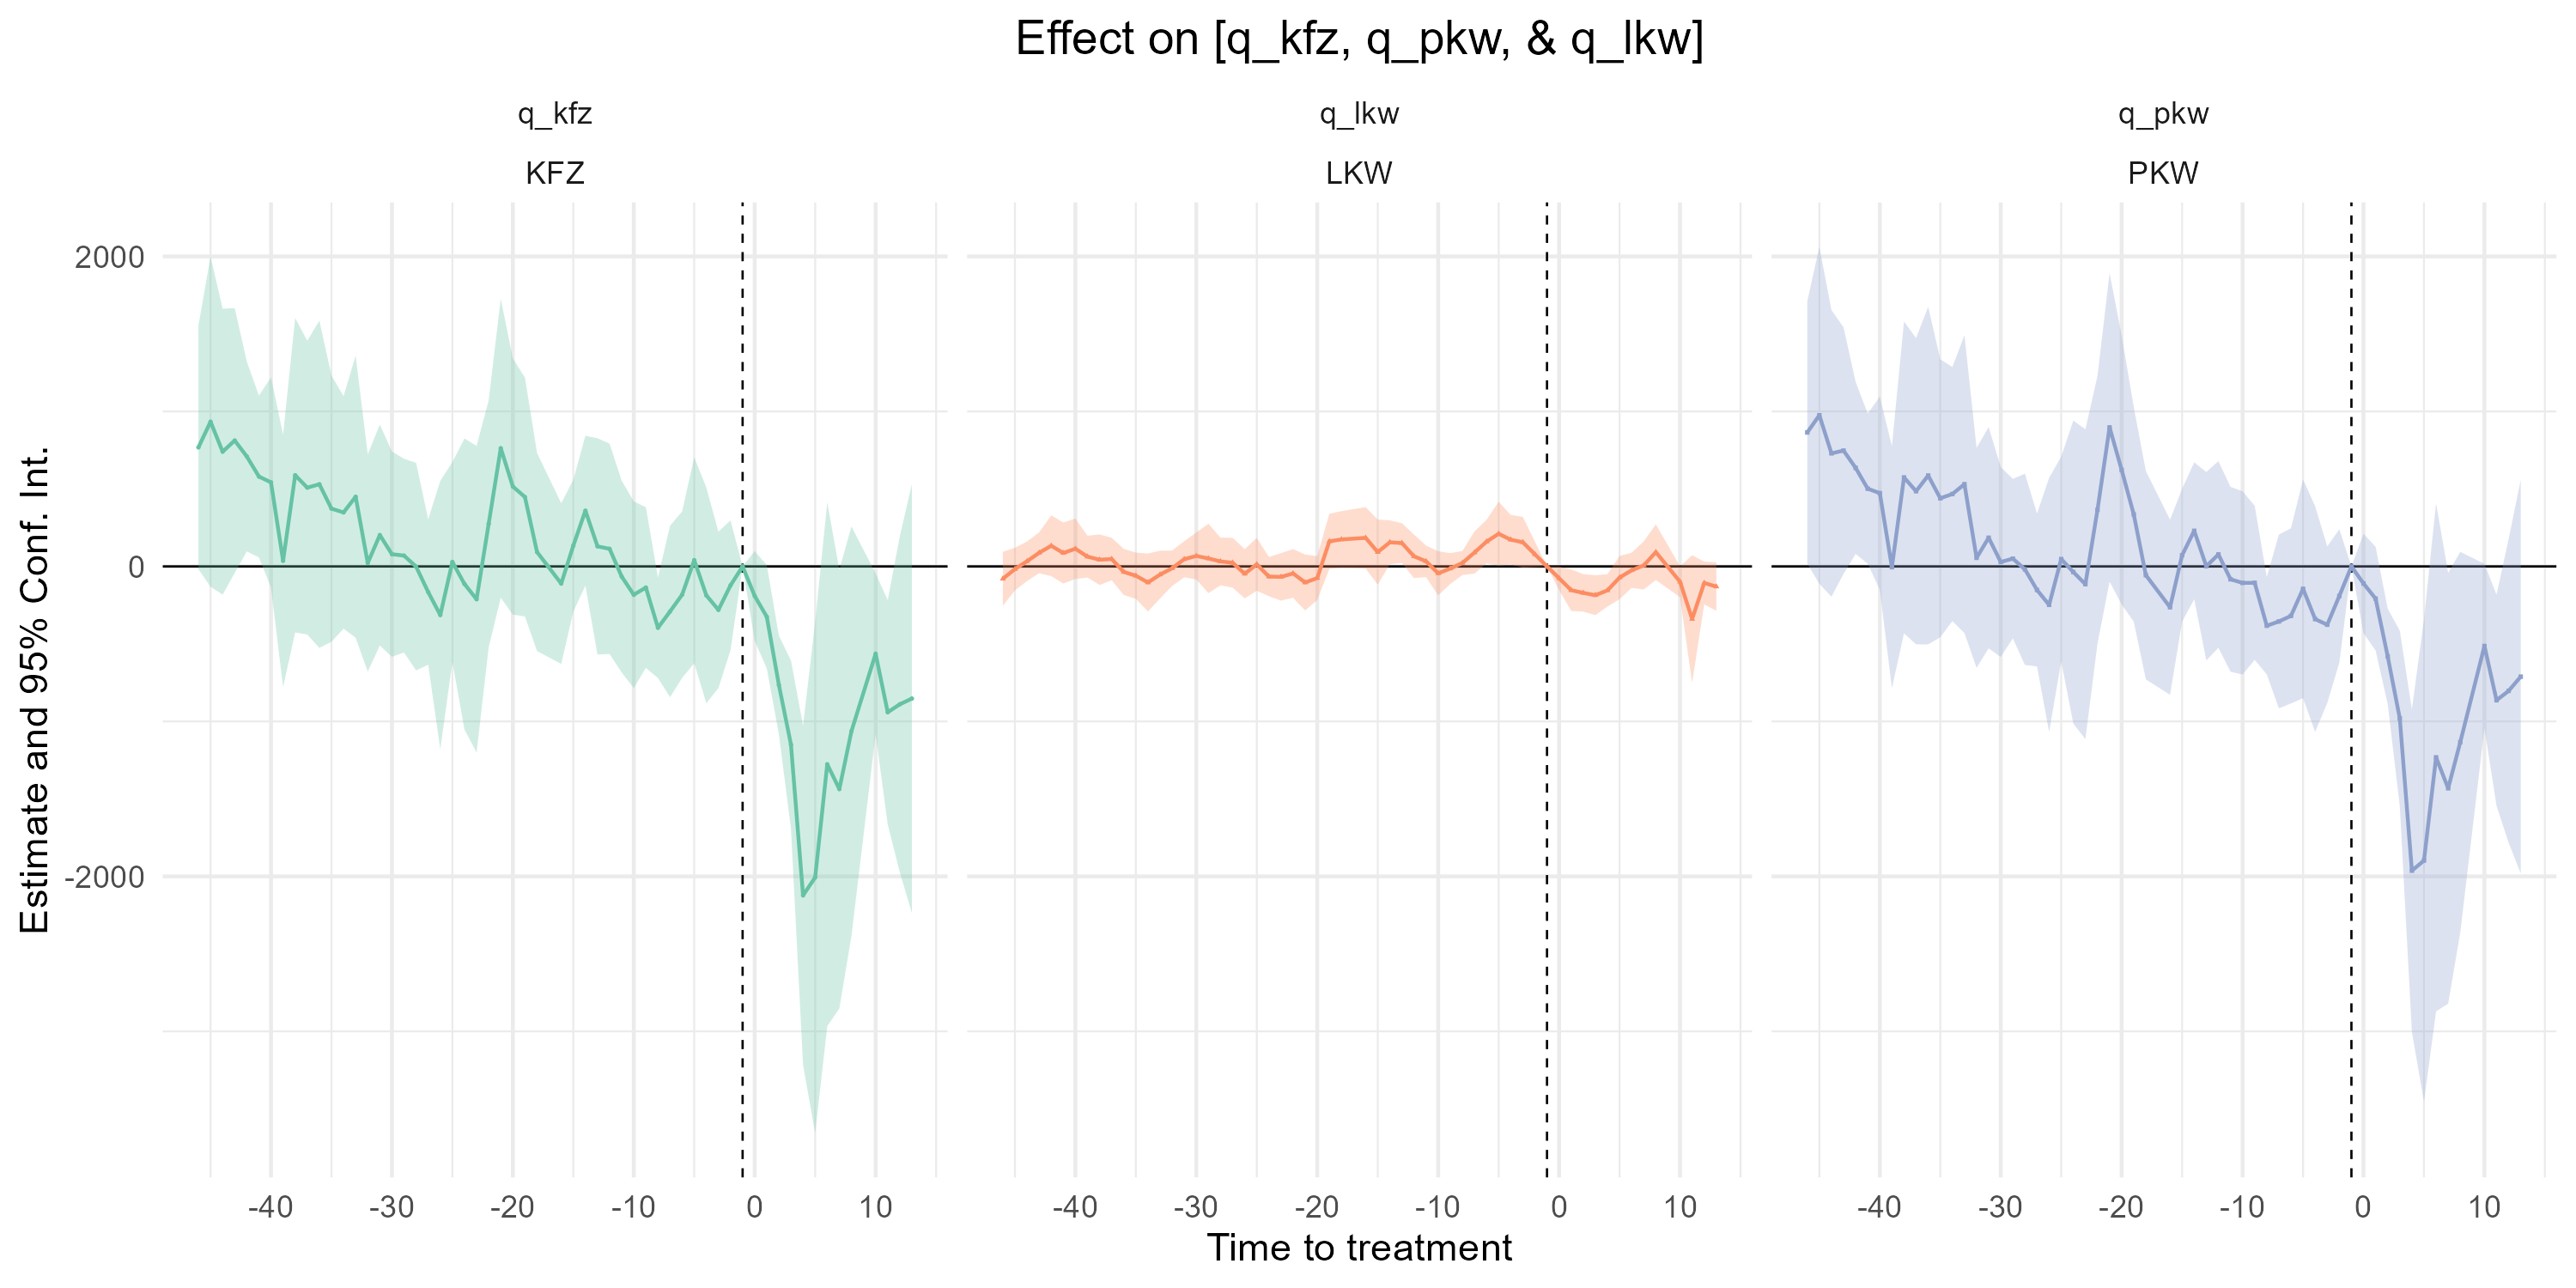
\includegraphics[width = \textwidth]{../04_figures/twfe_monthly_pt.png} 
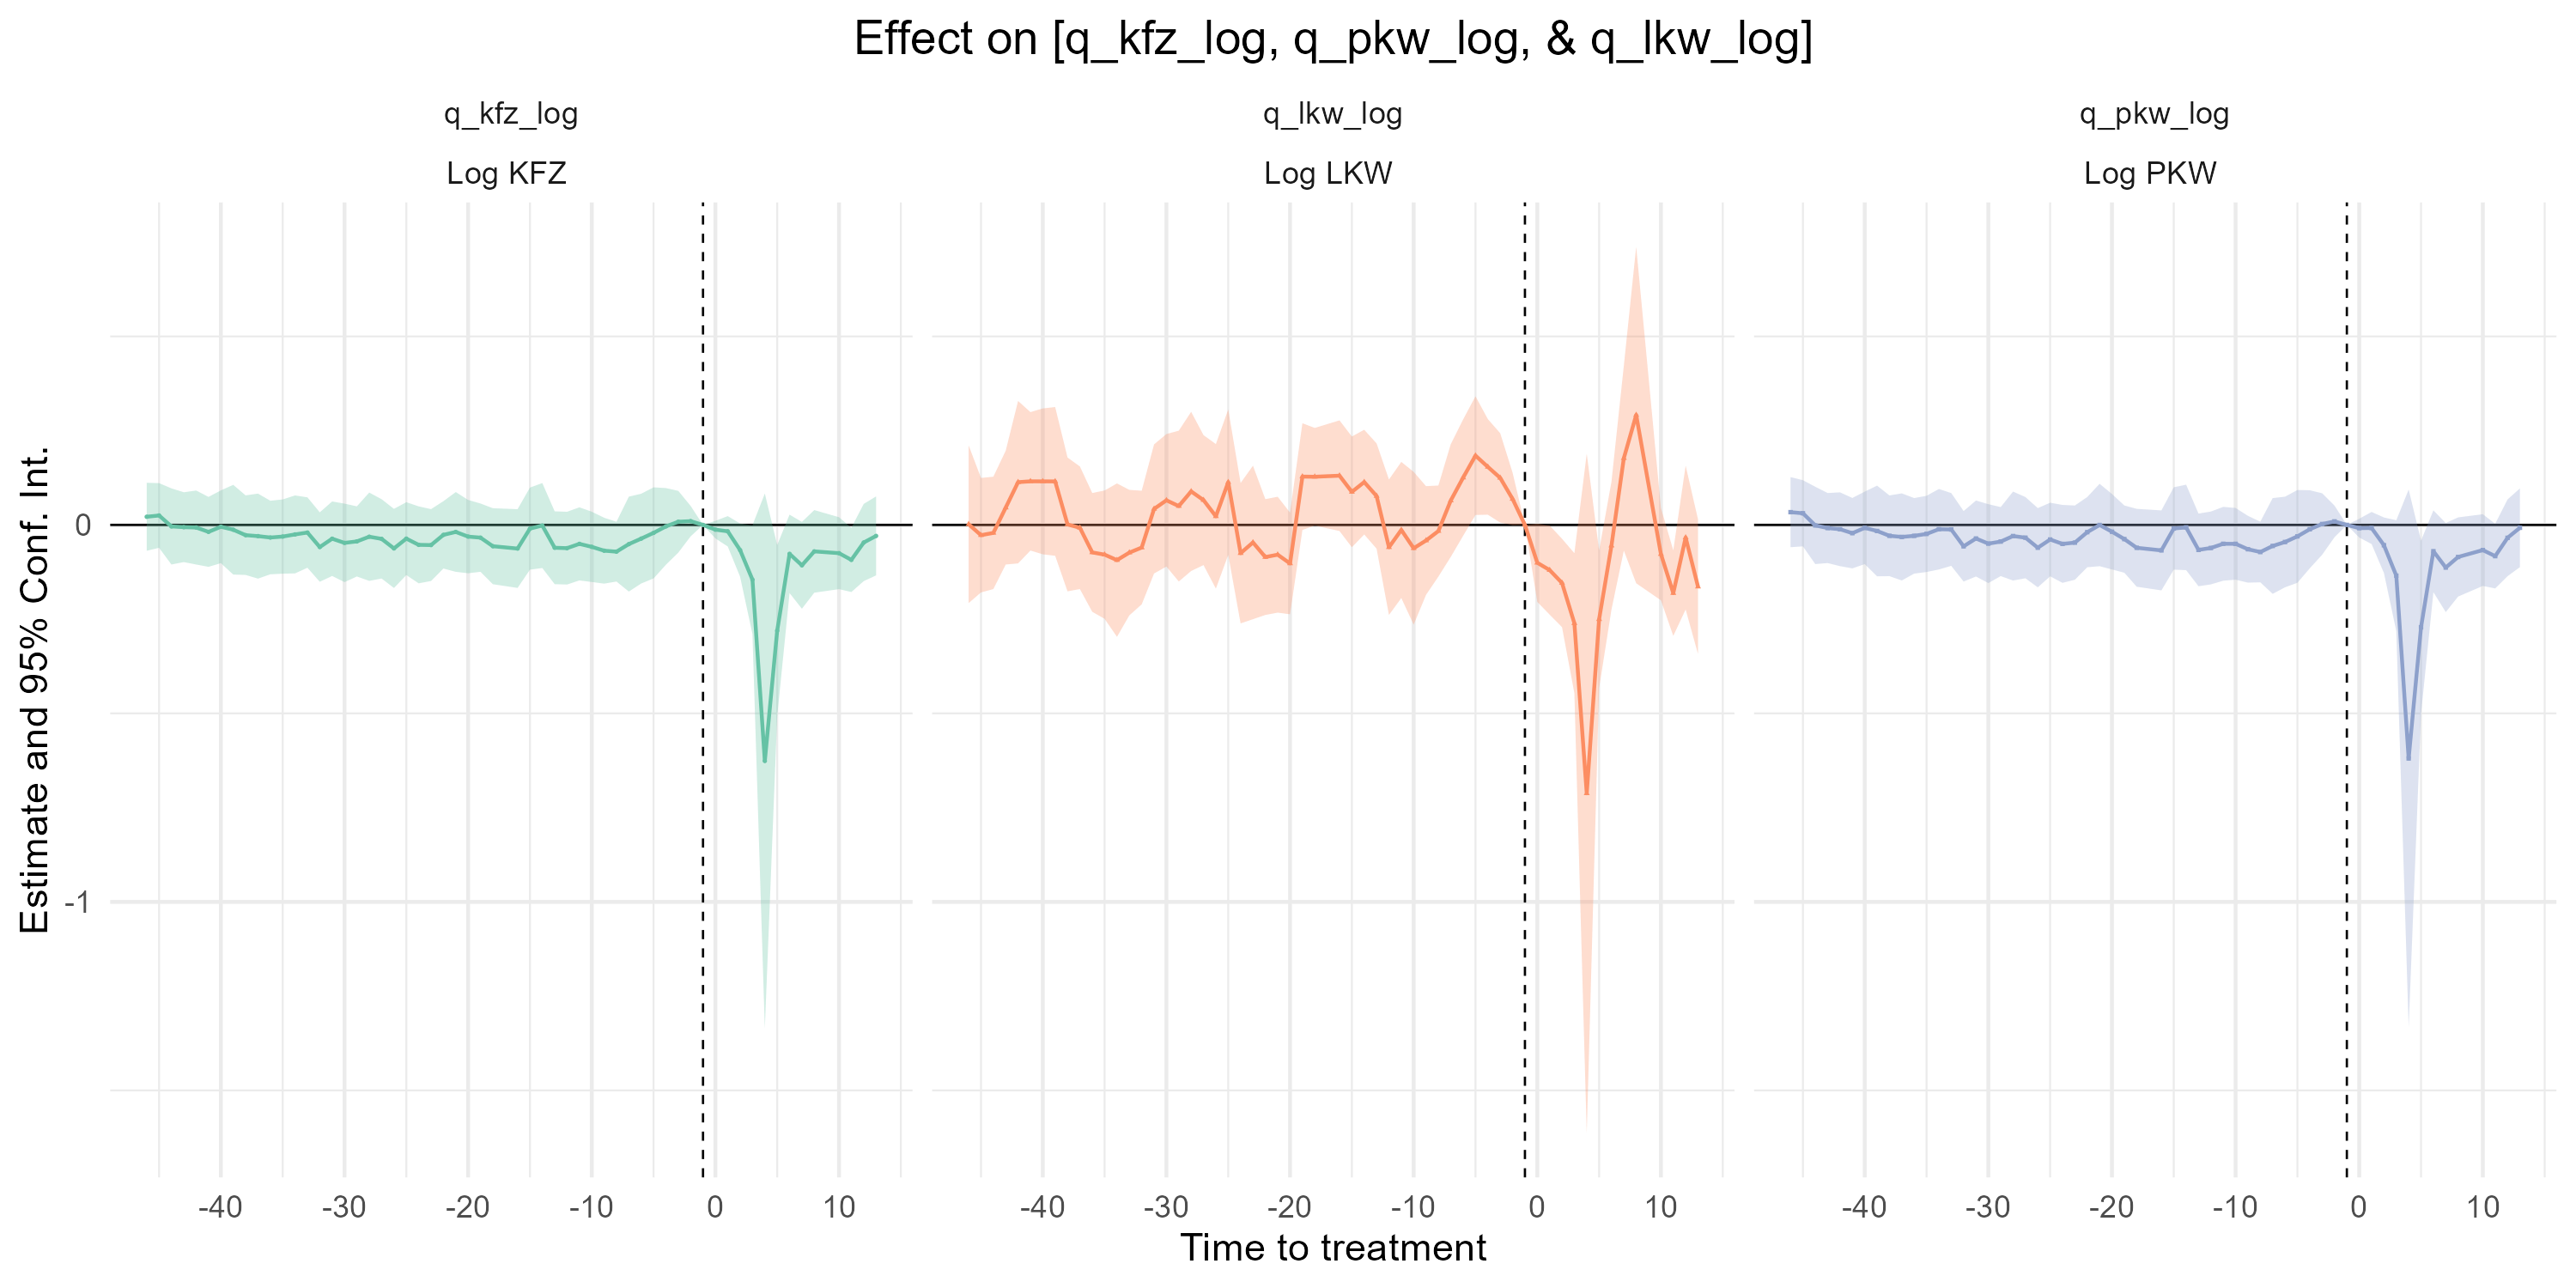
\includegraphics[width = \textwidth]{../04_figures/twfe_monthly_pt_log.png}
%\notes{rtreat - treatment radius; rbuffer - buffer radius; controls for temp., rain, sunshine, windspeed, rel. humidity with second order polynomials; monitor, year-month, and municipality-month FEs; 95\% CIs}
\end{figure}
%%
\begin{figure}[H]
\centering
\caption{Event study regressions via TWFE (w.o. Covid)}
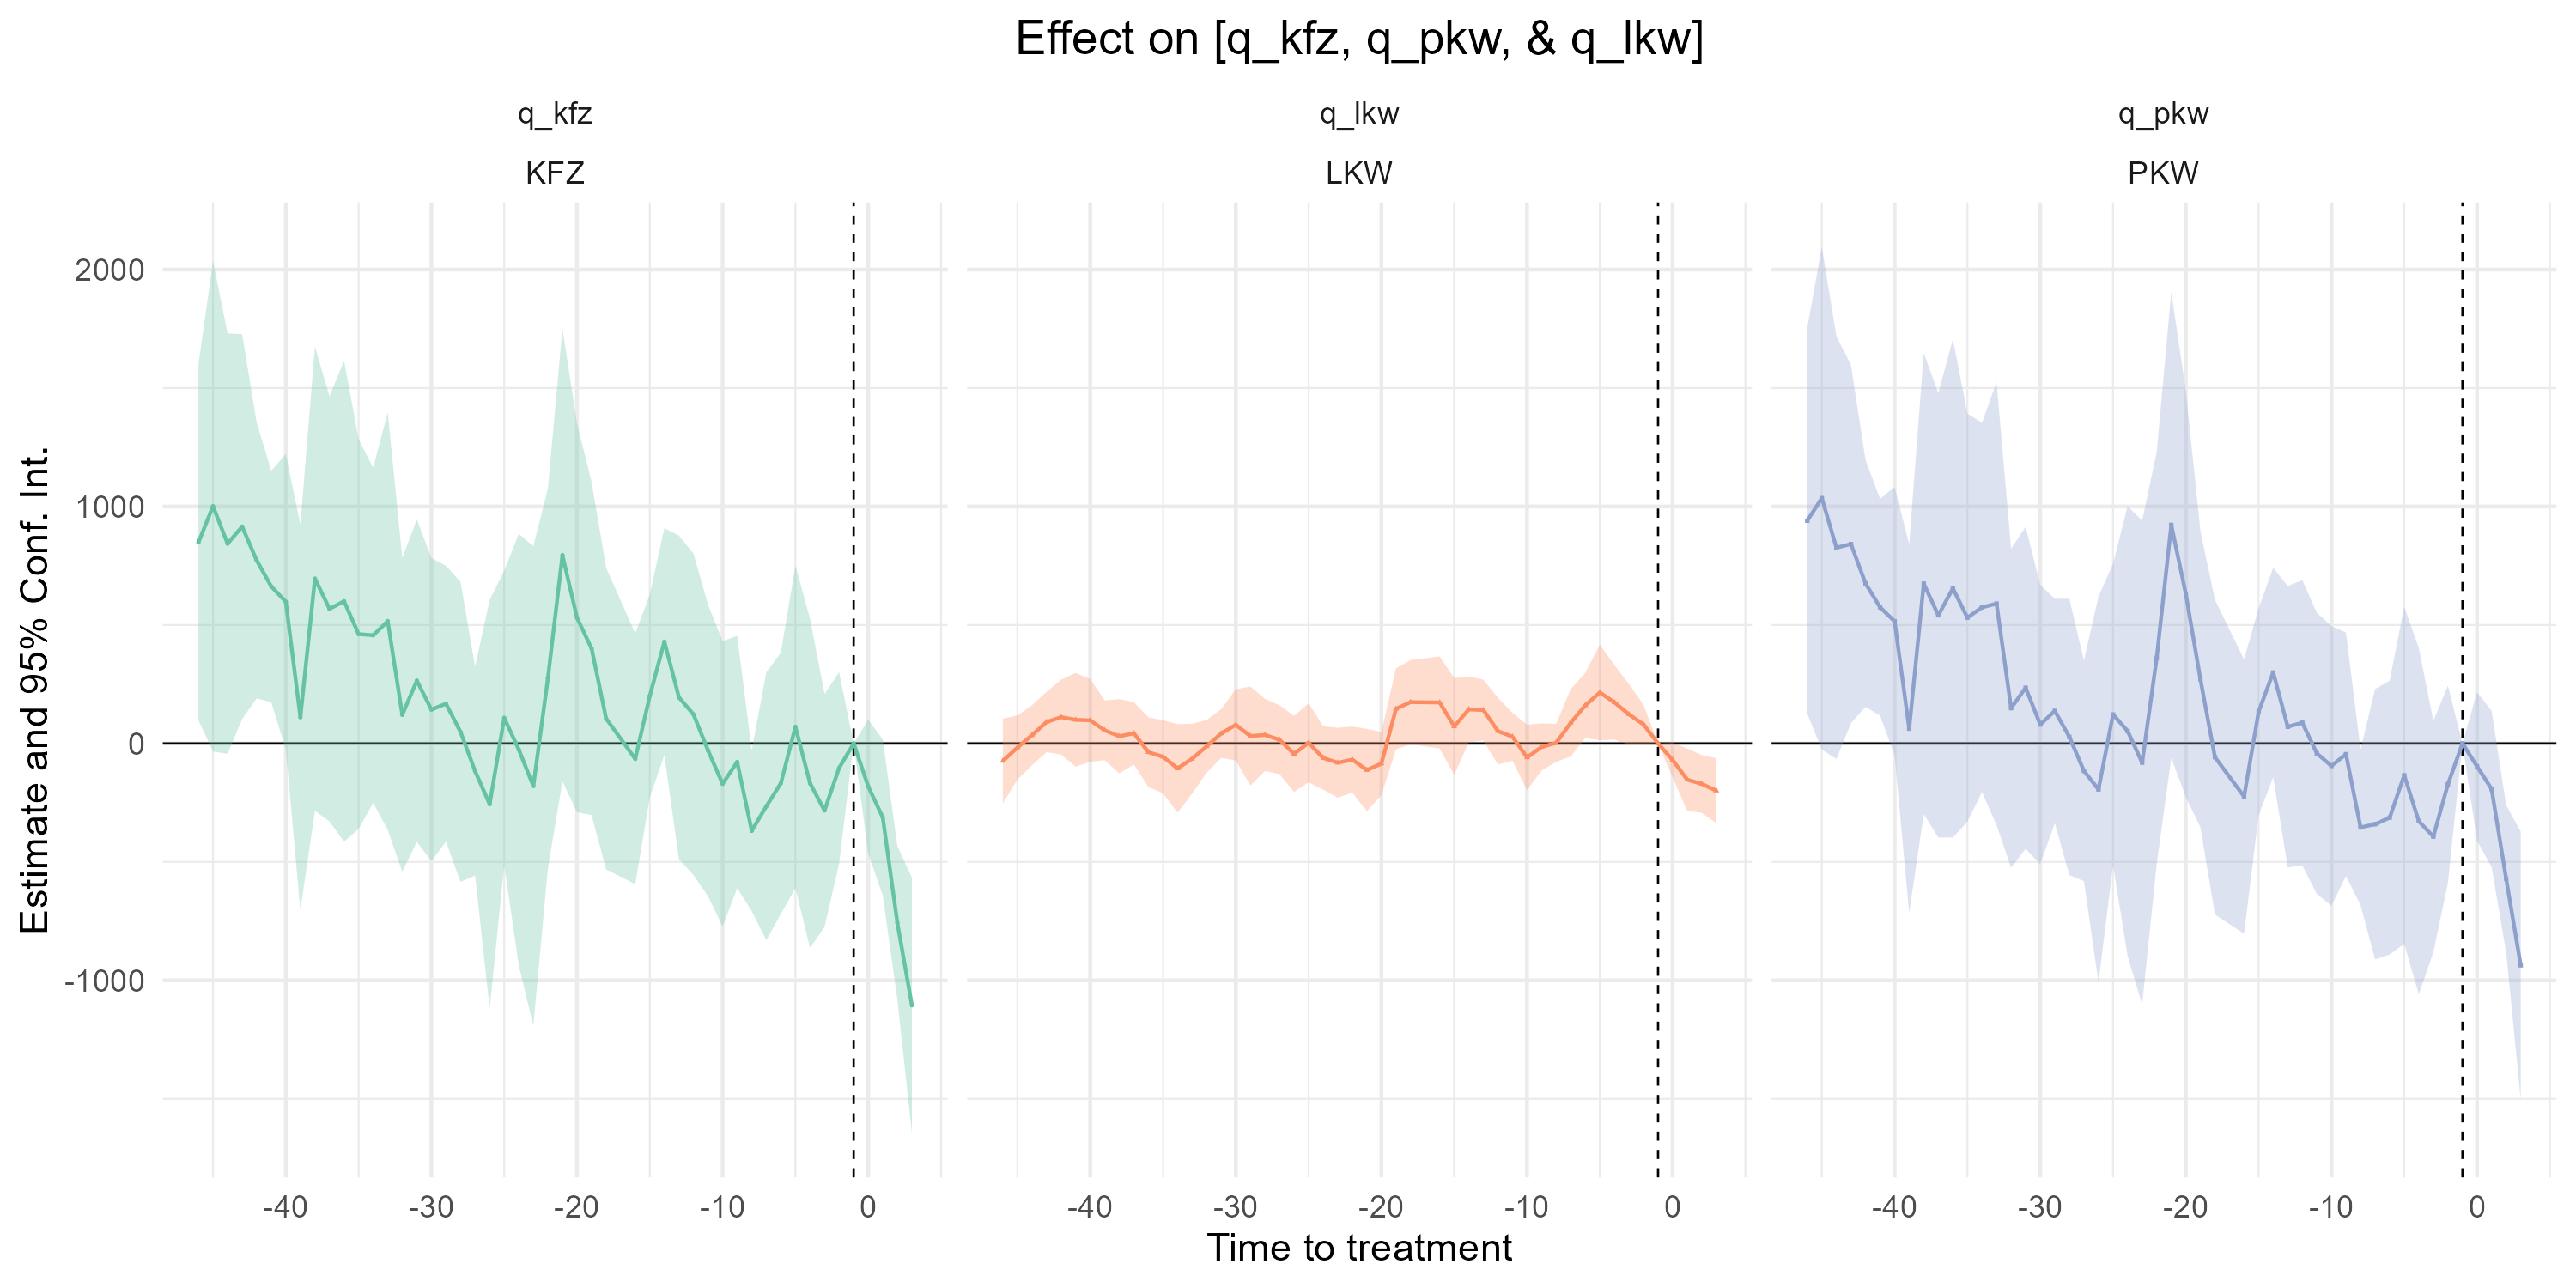
\includegraphics[width = \textwidth]{../04_figures/twfe_monthly_pt_lockdown.png} 
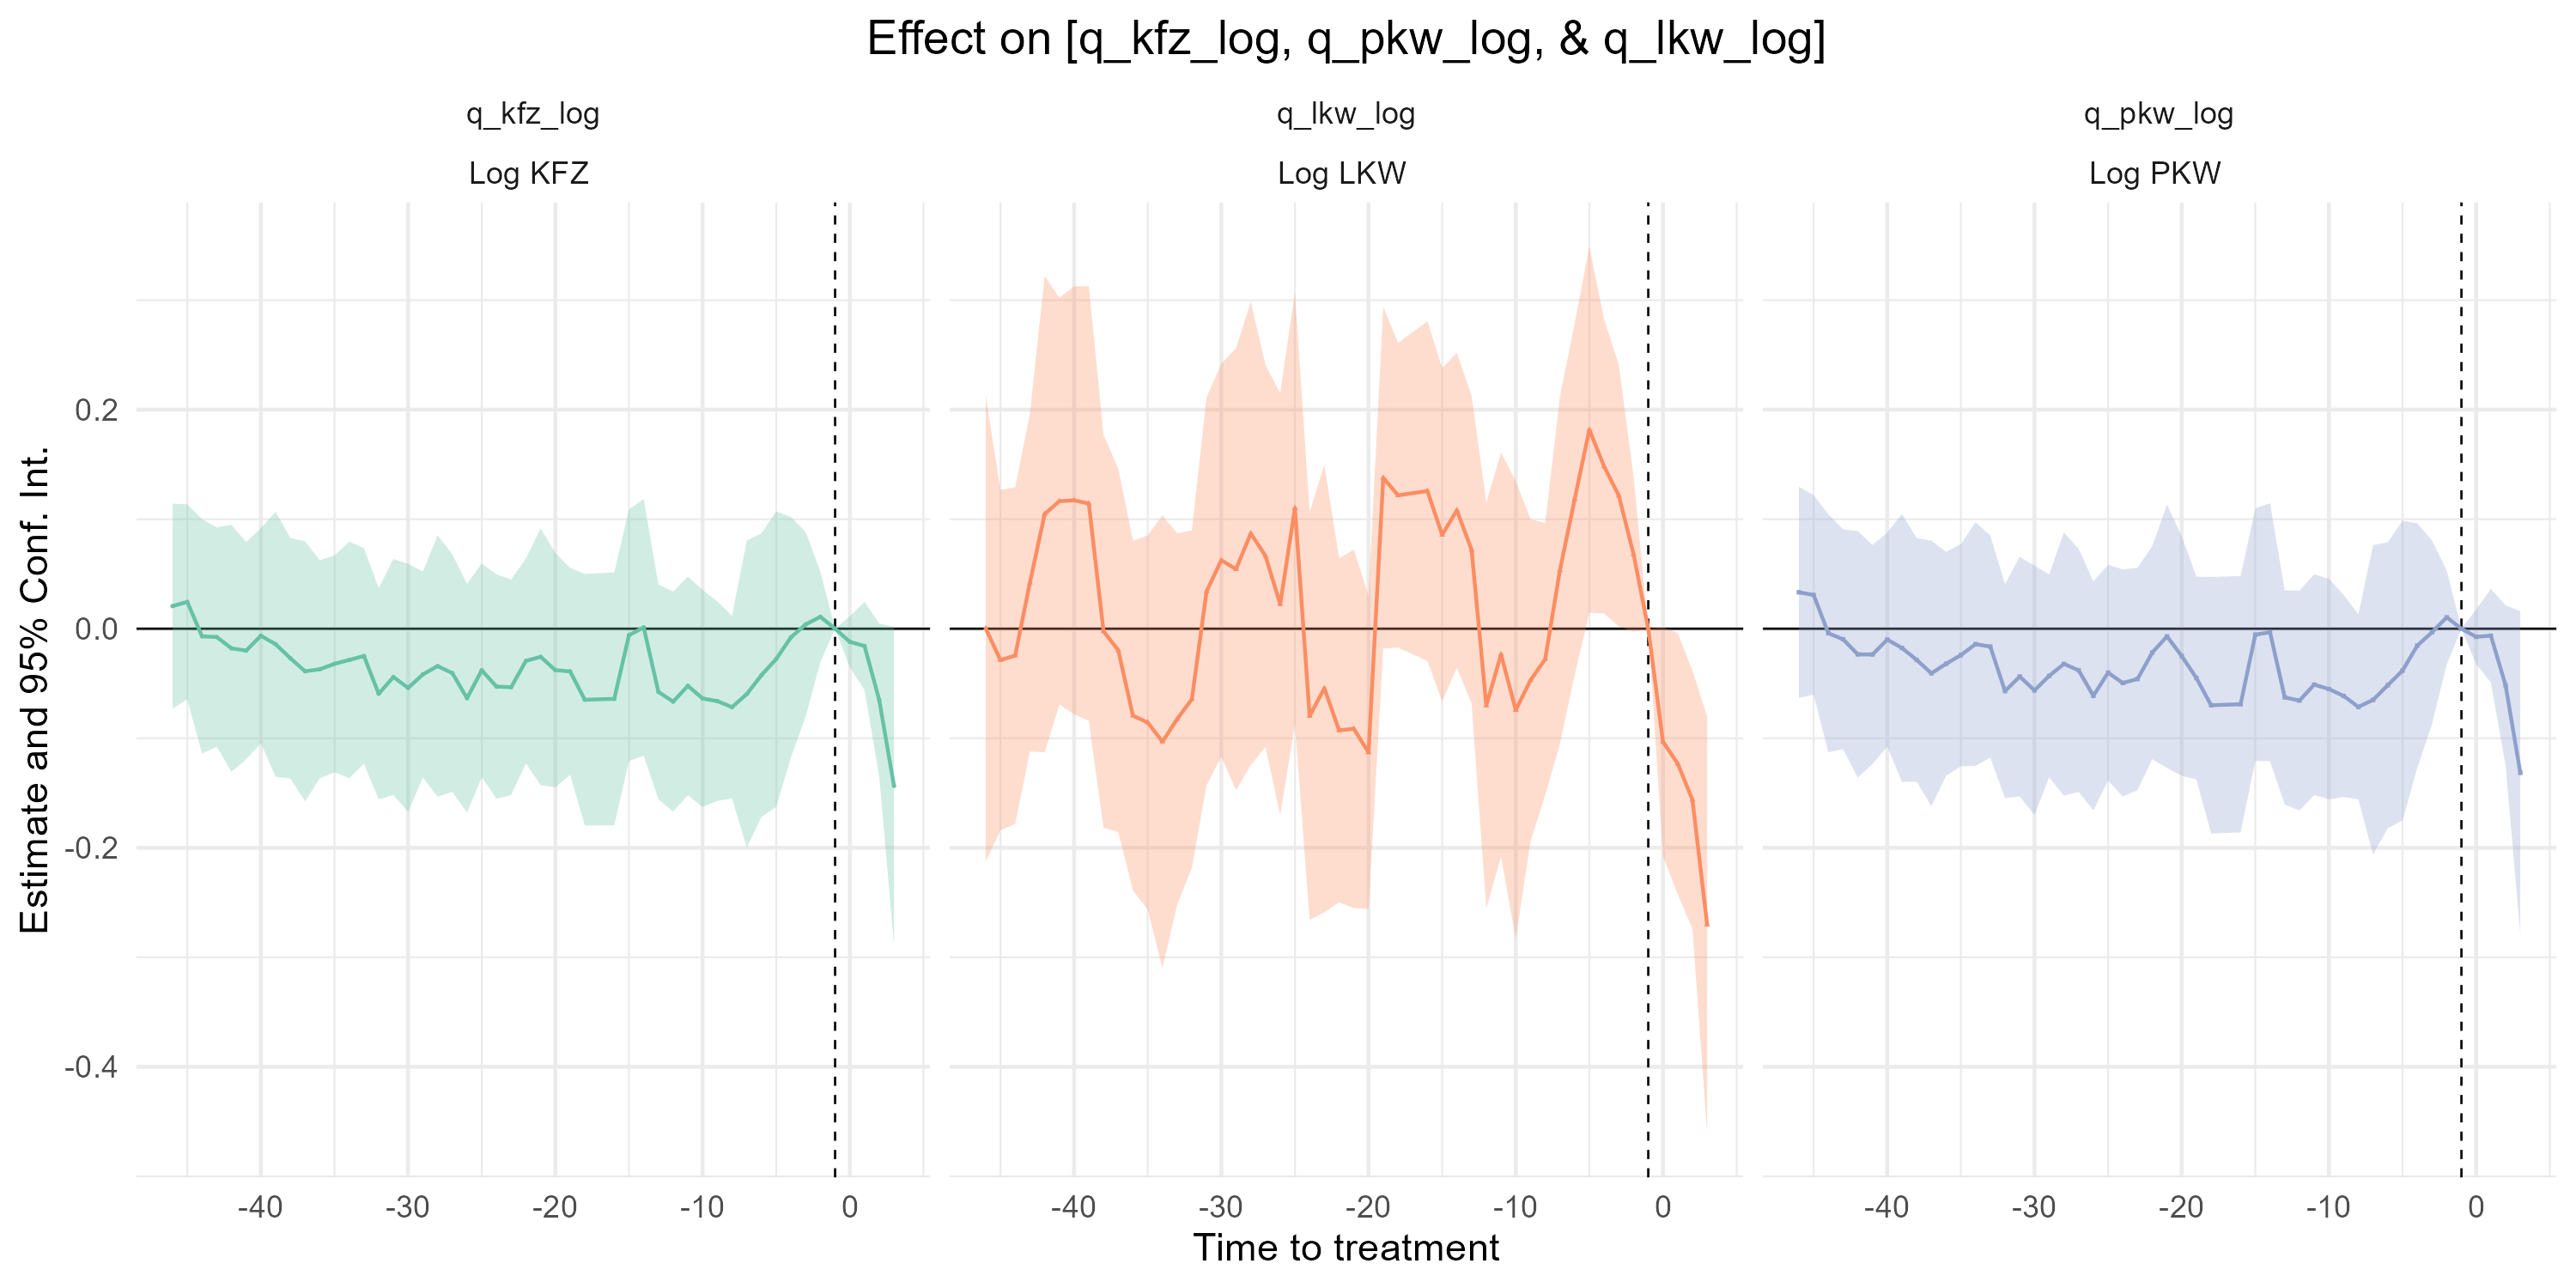
\includegraphics[width = \textwidth]{../04_figures/twfe_monthly_pt_log_lockdown.png}
%\notes{rtreat - treatment radius; rbuffer - buffer radius; controls for temp., rain, sunshine, windspeed, rel. humidity with second order polynomials; monitor, year-month, and municipality-month FEs; 95\% CIs}
\end{figure}

%\begin{figure}[H]
%\centering
%\caption{Event study regressions via Sun \& Abrahams}
%\includegraphics[width = \textwidth]{../04_figures/sab_monthly_pt.png} 
%\includegraphics[width = \textwidth]{../04_figures/sab_monthly_pt_log.png} 
%
%%\notes{rtreat - treatment radius; rbuffer - buffer radius; controls for temp., rain, sunshine, windspeed, rel. humidity with second order polynomials; monitor, year-month, and municipality-month FEs; 95\% CIs}
%\end{figure}
%%
%\begin{figure}[H]
%\centering
%\caption{Event study regressions via Sun \& Abrahams (w.o. Covid)}
%\includegraphics[width = \textwidth]{../04_figures/sab_monthly_pt_lockdown.png} 
%\includegraphics[width = \textwidth]{../04_figures/sab_monthly_pt_log_lockdown.png} 
%\end{figure}


\end{document}